\documentclass[a4paper, oneside,openany,12pt]{discothesis}

\usepackage[utf8]{inputenc}
\usepackage[spanish]{babel}
\usepackage[T1]{fontenc}
\usepackage{anysize}
\marginsize{4cm}{2cm}{3cm}{3cm}
\usepackage{perpage} %the perpage package
\MakePerPage{footnote} %footnote counting per page

%additional packages
\usepackage{graphicx}
\usepackage{physics}
\usepackage{tensor}
\usepackage{float}
\usepackage{bm}
\usepackage{siunitx}
\usepackage{multicol}
\usepackage{hyperref}
\usepackage{soul}
\usepackage{pgfgantt}
\usepackage{mathtools}
\usepackage{amsmath}
\usepackage{cancel}
\usepackage{enumitem}

%%%%%%%%%%%%%%%%%%%%%%%%%%%%%%%%%%%%%%%%%%%%%%%%%%%%%%%%%%%%%%%%%%%%%%%%%%%%%%%%%%%%%%%%%%%%%%%%%
% DOCUMENT METADATA

\thesistype{PROPUESTA DE TESIS PARA OPTAR AL TÍTULO DE FÍSICO} % Master's Thesis, Bachelor's Thesis, Semester Thesis, Group Project
\title{ESTRUCTURA ESTELAR Y ESTABILIDAD DE OBJETOS COMPACTOS CON UNA ECUACIÓN DE ESTADO NUMÉRICA}

\author{DAVID LEONARDO RAMOS SALAMANCA}
\email{}%david.ramos.salamanca@outlook.com}

\institute{%Grupo de Investigación en Relatividad y Gravitación  \\[2pt]
ESCUELA DE FÍSICA \\[2pt]
FACULTAD DE CIENCIAS \\[2pt]
UNIVERSIDAD INDUSTRIAL DE SANTANDER \\[2pt]
BUCARAMANGA \\[2pt]
2018}

% Optionally, you can put in your own logo here
%\logo{\includegraphics[width=0.4\columnwidth]{figures/uislogo}}

\supervisors{LUIS A. NÚÑEZ DE VILLAVICENCIO MARTÍNEZ}
%\cosupervisors{}


% Optionally, titleabs, authorabs, keywords and categories of the work can be shown (on the Abstract page)
\keywords{Estructura estelar, estabilidad,ecuación de estado numérica}
\titleabs{Estructura estelar de objetos compactos con una ecuación de estado numérica\footnote{Propuesta de trabajo de grado}} %Title for abstract
\authorabs{David Leonardo Ramos Salamanca\footnote{Facultad de Ciencias. Escuela de física. Director: Luis A. Núñez de Villavicencio Martínez}} %Author for abstract
%\categories{ACM categories go here.}

%Información para abstract en otro idioma----------------------- 
\keywordss{Stellar structure, stability, numerical equation of state}
\titleabss{Stellar structure and stability of compact objects with a numerical equation of state\footnote{Bachellor's thesis}} %Title for abstract
\authorabss{David Leonardo Ramos Salamanca\footnote{Facultad de Ciencias. Escuela de física. Adviser: Luis A. Núñez de Villavicencio Martínez}}

\date{\today}

%%%%%%%%%%%%%%%%%%%%%%%%%%%%%%%%%%%%%%%%%%%%%%%%%%%%%%%%%%%%%%%%%%%%%%%%%%%%%%%%%%%%%%%%%%%%%%%%%

\begin{document}

\frontmatter % do not remove this line
\maketitle

\cleardoublepage

%\begin{acknowledgements}
%	I thank Lorem ipsum dolor sit amet, consetetur sadipscing elitr, sed diam nonumy eirmod tempor invidunt ut labore et dolore magna aliquyam erat, sed diam voluptua. At vero eos et accusam et justo duo dolores et ea rebum. Stet clita kasd gubergren, no sea takimata sanctus est Lorem ipsum dolor sit amet. Lorem ipsum dolor sit amet, consetetur sadipscing elitr, sed diam nonumy eirmod tempor invidunt ut labore et dolore magna aliquyam erat, sed diam voluptua. At vero eos et accusam et justo duo dolores et ea rebum. Stet clita kasd gubergren, no sea takimata sanctus est Lorem ipsum dolor sit amet.
%\end{acknowledgements}


\begin{abstract}
    The abstract should be short, stating what you did and what the most important result is.
	Lorem ipsum dolor sit amet, consetetur sadipscing elitr, sed diam nonumy eirmod tempor invidunt ut labore et dolore magna aliquyam erat, sed diam voluptua. At vero eos et accusam et justo duo dolores et ea rebum. Stet clita kasd gubergren, no sea takimata sanctus est Lorem ipsum dolor sit amet. Lorem ipsum dolor sit amet, consetetur sadipscing elitr, sed diam nonumy eirmod tempor invidunt ut labore et dolore magna aliquyam erat, sed diam voluptua. At vero eos et accusam et justo duo dolores et ea rebum. Stet clita kasd gubergren, no sea takimata sanctus est Lorem ipsum dolor sit amet.\REMARK{¿Es necesario un abstract en la propuesta?}
\end{abstract}

\begin{abstract1}
    The abstract should be short, stating what you did and what the most important result is.
	Lorem ipsum dolor sit amet, consetetur sadipscing elitr, sed diam nonumy eirmod tempor invidunt ut labore et dolore magna aliquyam erat, sed diam voluptua. At vero eos et accusam et justo duo dolores et ea rebum. Stet clita kasd gubergren, no sea takimata sanctus est Lorem ipsum dolor sit amet. Lorem ipsum dolor sit amet, consetetur sadipscing elitr, sed diam nonumy eirmod tempor invidunt ut labore et dolore magna aliquyam erat, sed diam voluptua. At vero eos et accusam et justo duo dolores et ea rebum. Stet clita kasd gubergren, no sea takimata sanctus est Lorem ipsum dolor sit amet.
\end{abstract1}



\tableofcontents

\mainmatter % do not remove this line

% Start writing here-------------------------------------------

\chapter*{Introducción}
\addcontentsline{toc}{chapter}{Introducción}


\chapter{Estructura estelar}
\REMARK{The Development of the Theory of Stellar Structure}
\TODO{Breve introducción al capítulo más teórico de la tesis. Por qué es importante el estudio de la estructura estelar en equilibrio tanto en el caso newtoniano como en el relativista. Algo de historia de quienes desarrollaron lo que presento en el caso relativista y las condiciones de aceptabilidad física que se han establecido para discernir entre modelos. }

\section{Caso newtoniano}\TODO{Basado en los comentarios de la propuesta modificar esta sección}

Considerando una distribución de materia con simetría esférica, si $r$ denota la distancia desde el centro de la configuración, la masa encerrada en una superficie esférica de radio $r$ será:  
\begin{equation}
    m ( r ) = \int _ { 0 } ^ { r } 4 \pi r ^ { 2 } \rho \dd{r} = \int_{0}^{r} \dd{m(r)} \quad\text{con}\quad \dd{m(r)}=4\pi r^2\rho \dd{r},
    \label{mN}
\end{equation}

\begin{equation}
    \Longrightarrow\dv{m(r)}{r} =4\pi r^2 \rho.
    \label{dmnewton}
\end{equation}
Ahora, se considera un cilindro infinitesimal a una distancia $r$ del centro, de altura $\dd{r}$ y sección transversal unitaria, normal al vector posición $\vec{r}$ (ver Figura \ref{stellnew}).  

\begin{figure}[H]
    \centering
    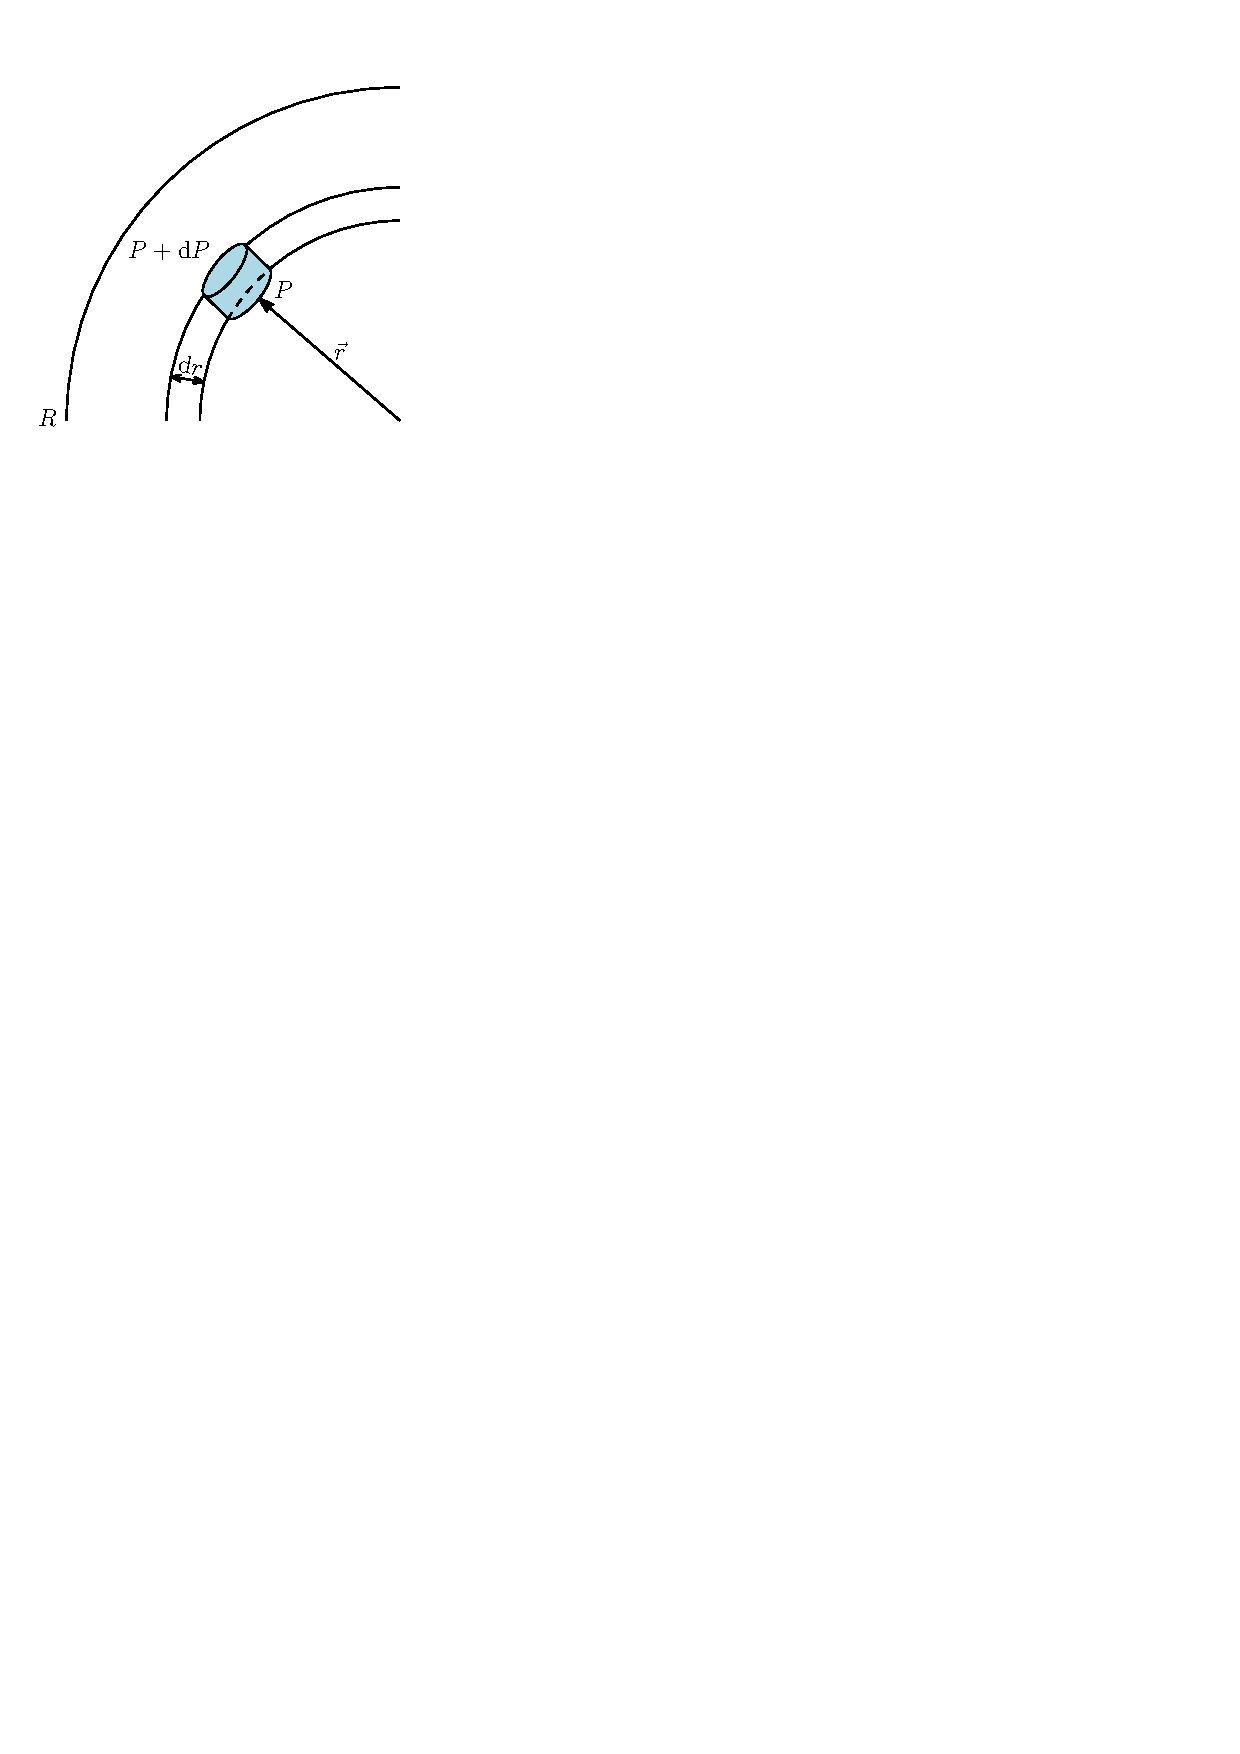
\includegraphics[width=150pt]{figures/stellarnewton.pdf}
    \caption{Presión sobre un elemento de masa cilíndrico.}
    \label{stellnew}
\end{figure}
Si la presión en $\vec{r}$ es $P$ y su cambio al ir de $\vec{r}$ a $\vec{r}+\dd{\vec{r}}$ es $\dd{P}$. Suponiendo que el elemento de área es $dA$ la diferencia de presión representa una fuerza 
\begin{equation*}
    F_{Pelem}=-\dd{P}\dd{A},
\end{equation*}
actuando sobre el elemento de masa. Esta fuerza debe contrarrestar la atracción gravitacional sobre el elemento de masa debido a $m(r)$
\begin{equation*}
    F_{atracc}=\frac{G m(r)\rho \dd{A} \dd{r}}{r^2}.
\end{equation*}
Para que el elemento de masa se encuentre en equilibrio se requiere entonces:

\begin{equation}
    -\dd{P}\dd{A} =\frac{G m(r)\rho \dd{A} \dd{r}}{r^2},
\end{equation}
o
\begin{equation}
    \dv{P}{r} = - \frac { G m ( r ) } { r ^ { 2 } } \rho.
    \label{dpnewton}
\end{equation}
que es la conocida ecuación de equilibrio hidrostático. 

Las ecuaciones \eqref{dmnewton} y \eqref{dpnewton} son las ecuaciones de estructura estelar newtonianas \cite{Chandrasekhar1958}. Si una relación entre la presión y la densidad $P(\rho)$ es dada, es decir, una ecuación de estado, el sistema puede resolverse dado un par condiciones iniciales $m(r=0)$ y $P(r=0)$. La primera de estas condiciones es evidente puesto que no hay masa encerrada en un cascarón esférico de radio nulo, $m(r=0)=0$. La segunda estará definida por el valor de $\rho(r=0)\equiv\rho_c$ escogido, mediante la ecuación de estado, $P(r=0)=P(\rho_c)$.

El radio de la estrella $R$ se define como el valor de $r$ en el que la presión se anula, esto es, $P(R)=0$ y de manera similar la masa de la estrella $M$ se define como el valor de la masa encerrada en $r=R$, esto es, $m(R)=M$.

\REMARK{Decidir si mantener o no} Aunque no se van a tratar en este trabajo, cabe resaltar que las \emph{enanas blancas} son bien descritas por las ecuaciones de estructura newtonianas. Una manera, aunque no la única, de conocer la importancia de las correcciones relativistas es comparando el valor de $\frac{2GM}{c^2R}$ con la unidad (la razón será evidente en el resultado relativista) \cite{Weinberg1972}. Las enanas blancas tienen masas en un rango de $0.33\,M_{\odot}$ $1.52\,M_{\odot}$ y radios típicos de unos cuantos miles de kilómetros \cite{Glendenning2000}. Para una enana blanca promedio, con masa $M=0.6\,M_{\odot}$ y radio $r=3000 \,\rm{km}$ se tiene
\begin{equation}
    \frac{2GM}{c^2R}\simeq 6\times 10^{-4}\ll 1,
\end{equation}
por lo cual se espera que el tratamiento newtoniano sea suficiente. 

\section{Caso relativista}\label{CR}\TODO{Basado en los comentarios de la propuesta modificar esta sección. Teniendo en cuenta que los cálculos están hechos en el apéndice.}

%Si bien en la teoría newtoniana podrían existir objetos tan compactos como las estrellas de neutrones, algunas de las predicciones presentan inconsistencias con lo predicho por la teoría de la Relatividad General. Por ejemplo, Chandrasekhar encontró (usando gravedad newtoniana) que las estrellas soportadas por presión de degeneración tienen una masa máxima, obtenida asintóticamente cuando los fermiones son altamente relativistas. Esto es, cuando tienen velocidades comparables con la velocidad de la luz. Bajo tales condiciones la teoría newtoniana permitiría la existencia de estrellas compuestas por los quarks más pesados (charm, bottom y top). En Relatividad General se predice también la existencia de una masa máxima, pero ésta no es de naturaleza asintótica sino que está inmersa en la forma de las ecuaciones de estructura estelar. Las estrellas con la mayor masa posible en Relatividad General, en contraste a lo predicho por la teoría newtoniana, no son lo suficientemente densas para permitir la presencia de los quarks más pesados \cite{Glendenning2000}.

%Predicciones contradictorias como la anterior favorecen a la Relatividad General en el estudio de objetos compactos, pues ésta ha explicado fenómenos como la precesión de mercurio, que no pueden ser explicados en gravedad newtoniana (ver  \cite{Turyshev2008ExperimentalRelativity} para una revisión de tests experimentales de la Relatividad General).

Para describir la estructura de una estrella estática en Relatividad General se supone un espacio-tiempo estático y con simetría esférica, descrito de manera general por el elemento de linea:

\begin{equation}
\dd{s}^ { 2 } = e ^ { 2 \nu ( r ) } \dd{ t} ^ { 2 } - e ^ { 2 \lambda ( r ) } \dd{ r} ^ { 2 } - r ^ { 2 } \left( \dd{ \theta} ^ { 2 } + \sin ^ { 2 }  \theta  \dd{ \phi} ^ { 2 } \right) .   
\end{equation}

La curvatura asociada a este elemento de linea (ver Apéndice A), debe satisfacer las ecuaciones de Einstein (en unidades gravitacionales ($G=c=1$))
\begin{equation}
    G _ { \mu } ^ { \nu }  = 8 \pi T _ { \mu } ^ { \nu },
\end{equation}
fijando así las funciones métricas $\nu$ y $\lambda$, en función del contenido material de la estrella descrito por $T _ { \mu } ^ { \nu }$.

Dividiendo el espacio-tiempo en dos: una región exterior a la estrella y una interior. 
La \textit{región exterior} está libre de fuentes ($T _ { \mu } ^ { \nu }=0$) y las ecuaciones de Einstein para ésta son 
\begin{equation}
    G _ { \mu } ^ { \nu } = 0.
\end{equation}
Este es un sistema de 3 ecuaciones, pues $ G _ { 2 } ^ { 2}=G _ { 3 } ^ { 3}$, y dos incógnitas. Por lo que una de las ecuaciones es redundante.
Restando las dos primeras ecuaciones
\begin{equation}
    G _ { 0 } ^ { 0} - G _ { 1 } ^ { 1} = -e^{-2\lambda} (\nu^{\prime}+\lambda^{\prime}) = 0 
\end{equation}
de donde
\begin{align}
    \nu^{\prime}+\lambda^{\prime} =& \,0 \\
    \int_{r}^{\infty} \qty(\dv{\nu}{r}+\dv{\lambda}{r})\dd{r} =& \,0 \\
    \eval{\nu}_{r}^{\infty} + \eval{\lambda}_{r}^{\infty} =& \, 0,
\end{align}
como $\lim_{r\to \infty}\nu(r)=\lim_{r\to \infty}\lambda(r)=0$
\begin{equation}
    \nu=-\lambda \quad \Longrightarrow \quad e^{2\nu}=e^{-2\lambda}. \label{metricfsschw}
\end{equation}
Integrando ahora la primera ecuación
\begin{align}
    G _ { 0 } ^ { 0} = -\frac{1}{r^{2}}+e^{-2\lambda}\left(\frac{1}{r^{2}}-\frac{2 \lambda^{\prime}}{r}\right) =& 0 \\
    e^{-2\lambda}\left(1-2 \lambda^{\prime} r \right) =& 1 \\
    \frac{d\left(r e^{-2 \lambda}\right)}{d r} =& 1 \\ 
    r e^{-2 \lambda} =& r - 2 M \\
    e^{2 \lambda} =& \left(1-\frac{2 M}{r}\right)^{-1},
\end{align}
donde $M$ es una constante de integración, y usando \eqref{metricfsschw} se obtiene
\begin{equation}
    e^{2\nu}=1-\frac{2 M}{r}.
\end{equation}

donde $M$ es una constante de integración interpretada como la masa de la estrella. Esta es la conocida solución exterior de Schwarzschild
\begin{equation}
    \dd{s} ^ { 2 } =  \left( 1 - \frac { 2 M } { r } \right) \dd{t} ^ { 2 } - \left( 1 - \frac { 2 M } { r } \right) ^ { - 1 } \dd{r} ^ { 2 }  - r ^ { 2 } \dd{\theta} ^ { 2 } - r ^ { 2 } \sin ^ { 2 } \theta \dd{\phi} ^ { 2 }, \label{schwarzs}
\end{equation}
valida para $r>R$, donde $R$ es el radio de la estrella, que describe la geometría del espacio-tiempo por fuera de una estrella estática.

Para la \textit{región interior} el contenido material debe ser especificado para resolver las ecuaciones de Einstein. Si la materia se modela como un fluido perfecto, el tensor de energía-momento viene dado por

\begin{equation}\label{EMT}
    \begin{array} { c } { T ^ { \mu \nu } = - P g ^ { \mu \nu } + ( P + \rho ) u ^ { \mu } u ^ { \nu } }, \\ \text{con} \quad { g _ { \mu \nu } u ^ { \mu } u ^ { \nu } = 1 }, \end{array}
\end{equation}
donde $u^{\mu}=\dv{x^{\mu}}{\tau}$ es la cuadri-velocidad de un elemento del fluido. Este tensor puede ser escrito en términos de los valores Minkowskianos de presión $P$ y densidad de energía $\rho$ gracias al Principio de Covariancia (consecuencia del Principio de Equivalencia \cite{Weinberg1972}), que permite escribir el tensor energía-momento en presencia de campos gravitacionales de una manera análoga a como se escribe en relatividad especial en ausencia de gravedad.

Como se considera una estrella estática, la velocidad espacial de todos los elementos del fluido son cero:
\begin{equation}
    u^{i}=0 \quad (i=1,2,3)\qc u ^ { 0 } = 1 / \sqrt { g _ { 00 } }
\end{equation}
con lo que las únicas componentes no nulas del tensor energía-momento, en componentes mixtas, serán

\begin{equation}
T _ { 0 } ^ { 0 } = \rho(r) , \quad T _ { i } ^ { i } = - P(r) \quad ( i=1,2,3 ).  
\end{equation}

Teniendo en cuenta la forma del tensor energía-momento, las ecuaciones de Einstein,

\begin{equation}
    G _ { \mu } ^ { \nu } = 8 \pi T _ { \mu } ^ { \nu },
\end{equation}
serán (ver Apéndice A)

\begin{equation}
    \begin{array} { l } { G _ { 0 } ^ { 0 } = e ^ { - 2 \lambda } \left( \frac { 1 } { r ^ { 2 } } - \frac { 2 \lambda ^ { \prime } } { r } \right) - \frac { 1 } { r ^ { 2 } } = - 8 \pi  \rho ( r ) }, \\ { G _ { 1 } ^ { 1 } = e ^ { - 2 \lambda } \left( \frac { 1 } { r ^ { 2 } } + \frac { 2 \nu ^ { \prime } } { r } \right) - \frac { 1 } { r ^ { 2 } } = 8 \pi  P ( r ) }, \\ { G _ { 2 } ^ { 2 } = e ^ { - 2 \lambda } \left( \nu ^ { \prime \prime } + \nu ^ { \prime 2 } - \lambda ^ { \prime } \nu ^ { \prime } + \frac { \nu ^ { \prime } - \lambda ^ { \prime } } { r } \right) = 8 \pi  P ( r ) }, \\ { G _ { 3 } ^ { 3 } = G _ { 2 } ^ { 2 } = 8 \pi  P ( r ) }. \end{array}
    \label{eee}
\end{equation}
Definiendo la masa de Misner como
\begin{equation}
    m ( r ) \equiv 4 \pi \int _ { 0 } ^ { r } \rho ( r ) r ^ { 2 } \dd{r},
    \label{me}
\end{equation}
se puede eliminar las funciones métricas de \eqref{eee}, expresándolas en términos de $P$, $\rho$ y $m$ \TODO{Realizar esta demostración} para obtener 

\begin{equation}
    \dv{P}{r} = - \frac { [ P ( r ) + \rho ( r ) ] \left[ m ( r ) + 4 \pi r ^ { 3 } P ( r ) \right] } { r [ r - 2 m ( r ) ] },
    \label{dptov}
\end{equation}
que junto a \eqref{me}, escrita como

\begin{equation}
    \dv{m}{r} = 4 \pi r ^ { 2 } \rho(r),
    \label{dmtov}
\end{equation}
son las ecuaciones de estructura estelar relativista y son la reducción de las ecuaciones de Einstein para el interior de una estrella esférica y estática. Este sistema es conocido como las ecuaciones de Tolman-Oppenheimer-Volkoff (TOV).

A pesar de que la masa de Misner \eqref{me} tiene la misma forma que la masa newtoniana \eqref{mN}, \eqref{me} incluye la energía total (masa bariónica y energía gravitacional) encerrada dentro de la coordenada $r$. Por esta razón se refiere a $M=m(R)$ como la \emph{masa gravitacional} de la estrella ya que no existe una forma unívoca de calcular la masa dada una distribución de energía arbitraria. 

Re-escribiendo \eqref{dptov} como
\begin{equation}
    \dv{P}{r} =  - \frac { G  m ( r ) } { r ^ { 2 } } \rho ( r ) \left[ 1 + \frac { P ( r ) } {c ^ { 2 } \rho ( r ) } \right] \left[ 1 + \frac { 4 \pi r ^ { 3 } P ( r ) } { m ( r ) c ^ { 2 } } \right]  \left[ 1 - \frac { 2 G m ( r ) } { c ^ { 2 } r } \right] ^ { - 1 }, 
    \label{dprelat}
\end{equation}
donde se revirtió el cambio de unidades, se puede reconocer como una versión relativista de la ecuación de equilibrio hidrostático newtoniana \eqref{dpnewton}. Las cuales coinciden en el límite cuando 
\begin{equation}
    c^2\rho \gg P \qc mc^2 \gg 4\pi r^3P \quad \text{y} \quad  \frac{2Gm}{c^2r}\ll 1,
\end{equation}
debido a que $P$ varia como $\frac{1}{2}mv^2$, las dos primeras condiciones se cumplen para velocidades pequeñas comparadas con la velocidad de la luz y se identifican los dos primeros términos de la ecuación \eqref{dprelat} como correcciones de relatividad especial.

Así pues, \eqref{dprelat} expresa el \textit{balance} entre la fuerza neta sobre un elemento de masa debido a la presión de la materia que la rodea y la atracción gravitacional de la materia interior a este. Además, como los tres factores en la ecuación \eqref{dprelat} son mayores que 1, se tiene que la atracción gravitacional aumenta en relatividad general, a medida de que $P$ se vuelve comparable con $\rho$ los gradientes de presión necesarios para sostener la estrella aumentan hasta que el colapso es inevitable.\TODO{Refinar argumento.}

%Así pues,  \eqref{dprelat} expresa el \textit{balance} entre la fuerza neta sobre un elemento de masa debido a la presión de la materia que la rodea y la atracción gravitacional de la materia interior a este. Los tres factores en la ecuación \eqref{dprelat} son mayores que 1, esto es, además de la densidad de energía, la presión actúa como una fuente de atracción gravitacional. Esta es la razón por la cual el colapso gravitacional es intrínseco a la estructura de la Relatividad General: mientras en las estrellas newtonianas la presión actuaba para sostener a la estrella, si la estrella es lo suficiente masiva (presiones lo suficientemente grandes) el colapso es inevitable.

Las ecuaciones de TOV \eqref{dptov} y \eqref{dmtov}, pueden ser resueltas de manera análoga a las ecuaciones de estructura newtonianas. Dada una ecuación de estado $P(\rho)$ y partiendo de las condiciones iniciales $m(r=0)=0$ y $P(r=0)=P(\rho_c)$, el sistema se puede integrar hasta que la presión se anule, lo que indica el borde de la estrella y define el radio $R$ y la masa gravitacional $m(R)=M$ de la estrella. Los modelos de objetos compactos obtenidos dada cierta ecuación de estado forman una familia parametrizada por la densidad central $\rho_c$. Algunas características generales de la ecuación de estado serán descritas en la siguiente sección.

La función métrica $\nu$ puede ser hallada añadiendo al sistema la ecuación diferencial

\begin{equation}
    \dv{\nu}{r} = \frac { m ( r ) + 4 \pi r ^ { 3 } P ( r ) } { r [ r - 2 m ( r ) ] },
\end{equation}
cuya solución debe coincidir con la solución externa en $R$, por lo que se usa la libertad de sumar una constante para realizar el siguiente cambio
\begin{equation}
    \nu ( r ) \longrightarrow \nu ( r ) - \nu ( R ) + \frac { 1 } { 2 } \ln \left( 1 - \frac { 2 M } { R } \right) , \quad r \leq R.
\end{equation}
Sujeta a una condición inicial, generalmente $\nu(r=0)=0$\TODO{Revisar si en serio no es posible usar esta condición}.



\section{Condiciones de aceptabilidad física}
Para que los modelos de objetos compactos obtenidos sean de interés astrofísico, las variables físicas y métricas deben cumplir con varias condiciones de regularidad, acoplamiento y estabilidad. Estas condiciones fueron recopiladas recientemente por B. V. Ivanov \cite{Ivanov2017} y extendidas por Nuñez et al. \cite{Hernandez2018}, a continuación se presentará una deducción/justificación de estas condiciones. 

\subsection*{Sobre las funciones métricas}
\textbf{C1:} Las funciones métricas son positivas y deben ser finitas y libres de singularidades en el interior de la estrella.
\TODO{¿Razones físicas de esto?}
\subsection*{Condiciones de acoplamiento}\TODO{Verificar si de C3 se llega a continuidad de 1ra forma fund.}
 Para acoplar la solución interior y exterior sobre la superficie de la estrella, es necesario imponer condiciones de acoplamiento de modo que el espacio-tiempo este bien definido. 
 La formulación de estas condiciones usadas con mayor frecuencia fueron desarrolladas por Darmois\TODO{Cita.}\, y se basa en consideraciones sobre la curvatura intrínseca y extrínseca de la 3-superficie $\Sigma$ tipo tiempo que describe la superficie de la estrella.
 
 Si $\vec{n}$ es el vector (tipo espacio) normal a $\Sigma$, se introducen coordenadas Gausianas donde $n=cte$ define 3-superficies tipo tiempo vecinas a $\Sigma$ (ver Figura \ref{JC}). La métrica en estas coordenadas tiene la forma 
 \begin{equation}
g=(\vec{n} \cdot \vec{n})^{-1} d n\otimes d n +g_{i j} d x^{i} \otimes d x^{j}. 
\end{equation}

 \begin{figure}[H]
     \centering
     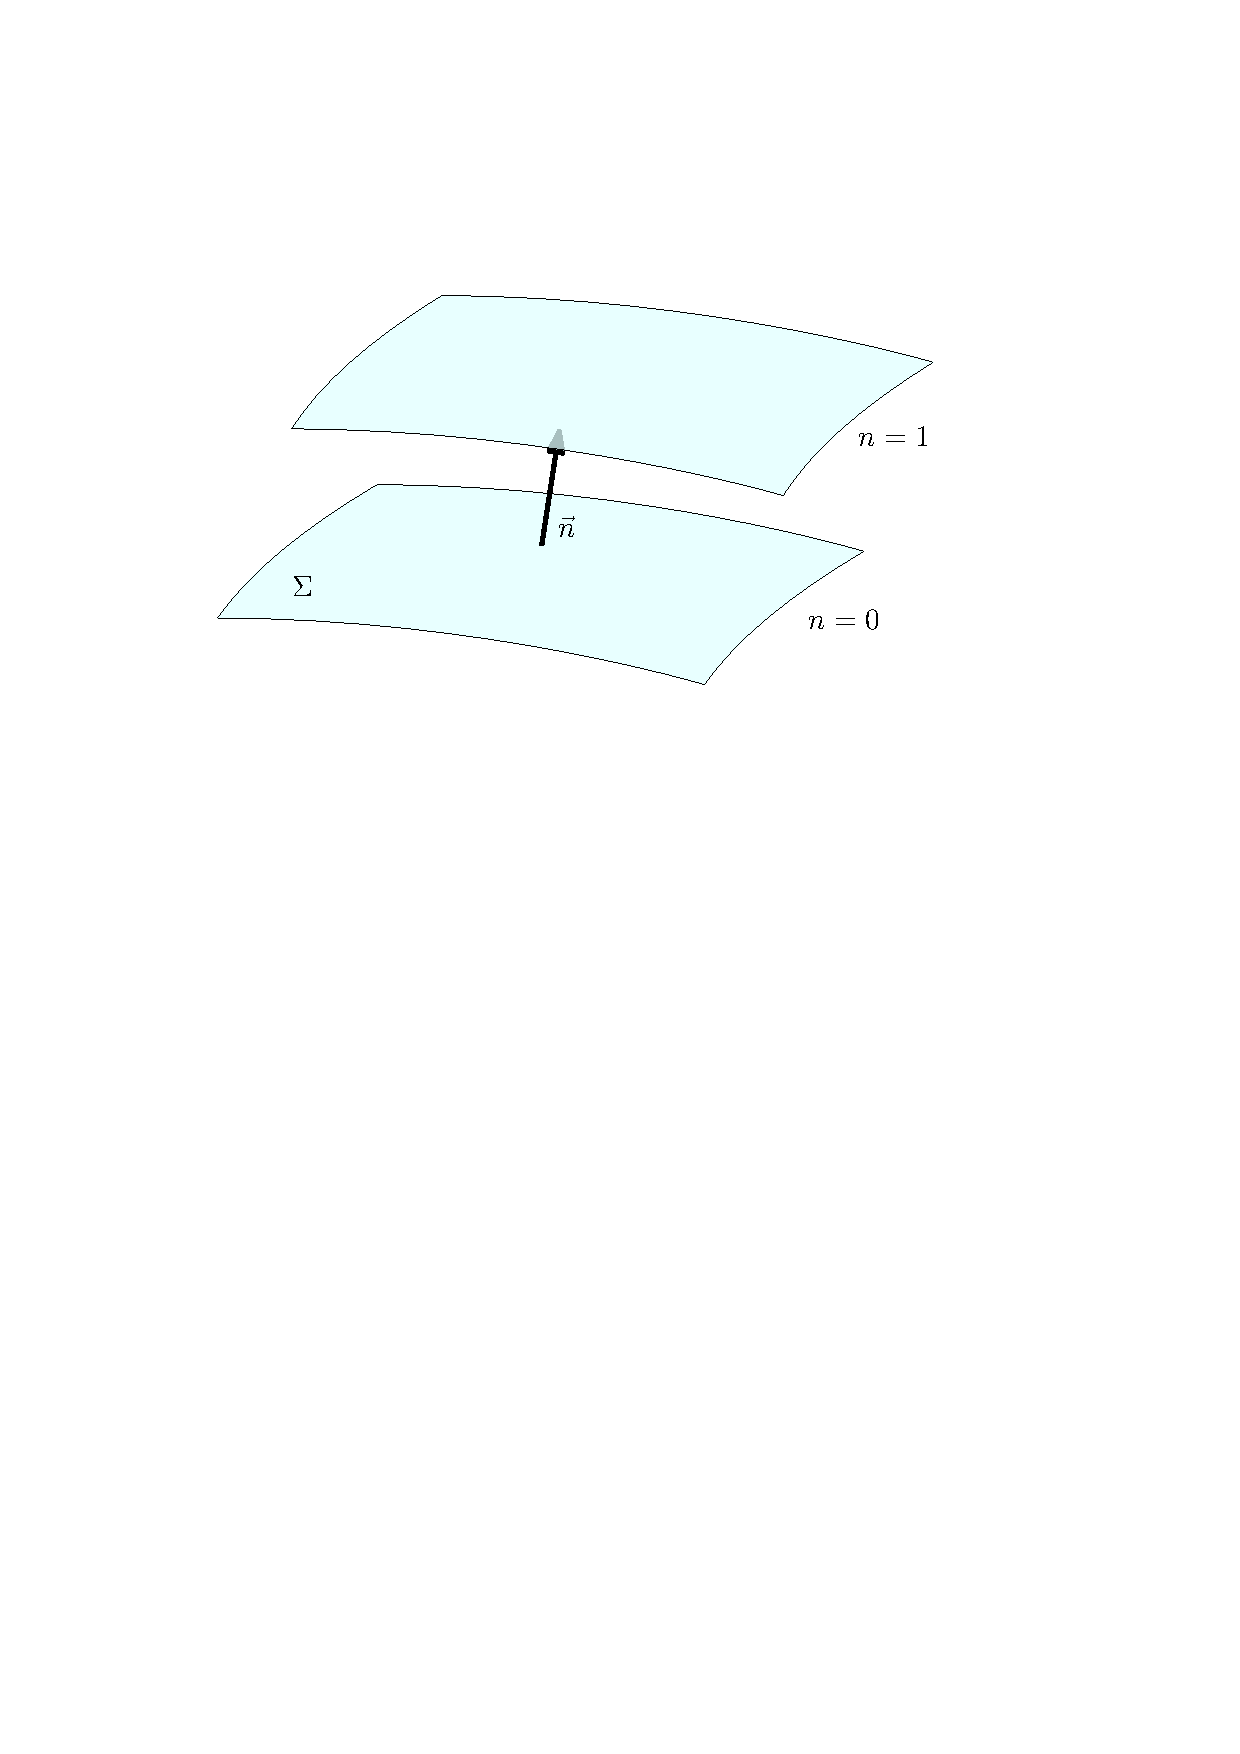
\includegraphics[width=0.7\linewidth]{figures/Junction.pdf}
     \caption{Coordenadas Gausianas en el vecindario a $\Sigma$}
     \label{JC}
 \end{figure}
Las condiciones de acoplamiento en este "set-up" son:
 \begin{enumerate}[leftmargin=2cm]
     \item La métrica inducida $g_{ij}$ es continua a través de $\Sigma$.
     \item El tensor de energía-momento superficial se anula en la superficie
     \begin{equation}
\lim _{\varepsilon \rightarrow 0}\left[\int_{-e}^{+\varepsilon} T_{\beta}^{\alpha} d n\right]=0.
    \end{equation}
     
 \end{enumerate}
 
 \textbf{C2:} Para el caso considerado en este trabajo $\Sigma:\,r=R$, además la simetría esférica permite identificar $\vec{n}=\pdv{r}$ y debido a que la solución externa es de vacío $\eval{T^{\alpha}_{\beta}}_{+\epsilon}$= 0, bajo estas condiciones las condiciones de acoplamiento se reducen a
 \begin{enumerate}[leftmargin=2cm]
     \item $e ^ {  2 \nu(R) } =  1 - \frac { 2 M } { R }$.
    \item $P(R)=\rho(R)=0$.
 \end{enumerate}


\subsection*{ Sobre el corrimiento al rojo gravitacional}
La luz emitida por una estrella es observada corrida al rojo por un observador lejano debido a la presencia del campo gravitacional. Qué tanto es corrida al rojo puede ser estimado de manera sencilla \cite{Glendenning2000}: considerando un átomo de la estrella a una distancia $r$ de su centro, que emite un fotones con determinada frecuencia, el intervalo de tiempo propio entre dos emisiones consecutivas está dado por
\begin{equation}
d \tau=\sqrt{-g_{\mu \nu} d x^{\mu} d x^{\nu}},
\end{equation}
en el marco del átomo esto es simplemente ($dx^i=0$)
\begin{equation}
d \tau_{\mathrm{e}}=\sqrt{-g_{00}(r)} d t.
\end{equation}
Si suponemos que el observador y el átomo yacen sobre la misma línea el intervalo espacio-temporal para la radiación es
\begin{equation}
d \tau^{2}=g_{11}(r) d r^{2} - g_{00}(r) d t^{2} = 0,
\end{equation}
así que el tiempo que tardó un ciclo en viajar de $r$ a $\infty$ es
\begin{equation}
\Delta t=t_{\infty}-t_{R}=\int_{R}^{\infty}\left(\frac{g_{11}(r)}{g_{00}(r)}\right)^{1 / 2} d r,
\end{equation}
es decir, $dt$ (tiempo coordenado entre dos emisiones consecutivas) es el mismo para el emisor y el observador lejano. Con lo anterior, el tiempo propio para el observador será
\begin{equation}
d \tau_{\mathrm{o}}=\sqrt{-g_{00}(\infty)} d t.
\end{equation}
Como el inverso del tiempo propio es proporcional a la frecuencia, la razón entre la frecuencia emitida y observada es
\begin{equation}
\frac{\omega_{\mathrm{e}}}{\omega_{\mathrm{0}}}=\left(\frac{g_{00}(\infty)}{g_{00}(r)}\right)^{1 / 2}=e^{-\nu(r)},
\end{equation}
y con esto el corrimiento al rojo gravitacional es
\begin{equation}
    z(r)\equiv \frac{\omega_{\mathrm{e}}-\omega_{\mathrm{o}}}{\omega_{\mathrm{o}}}  = e^{-\nu(r)}-1.
    \label{redshift}
\end{equation}
\textbf{C3:} El corrimiento al rojo descrito por \eqref{redshift} debe disminuir con el incremento de $r$.
\subsection*{Sobre el signo de la densidad de energía y la presión}
La densidad de energía y la presión deben ser positivas dentro de la estrella.\TODO{Materia normal?}

\subsection*{Sobre la densidad de energía y la presión}
\textbf{C5:} La densidad de energía y la presión deben alcanzar un máximo en el centro ($\rho'(0)=P'(0)=0$) y deben decrecer monótonamente hacia afuera.\TODO{Decrecimiento monótono?}

\subsection*{Condiciones de energía}
Con el fin de obtener soluciones a las ecuaciones de Einstein en presencia de fuentes de energía y momento realistas es necesario imponer ciertas condiciones de energía que limiten la arbitrariedad del tensor energía-momentum escogido.

Existe una variedad de condiciones de energía que son usadas en diferentes circunstancias, las usadas con mayor frecuencia son \cite{Hawking1973TheSpaceTime,Carroll2003SpacetimeRelativity}:

\begin{itemize}[leftmargin=1.5cm]
    \item \emph{Condición de energía débil}: el tensor de energía-momentum en cada punto $p$ de la variedad obedece la desigualdad $T_{\mu \nu} t^{\mu} t^{\nu} \geq 0$ para cualquier vector tipo tiempo $t^{\mu}\in T_{p}$.
    \item \emph{Condición de energía dominante}: el tensor de energía-momentum en cada punto $p$ de la variedad obedece la desigualdad $T_{\mu \nu} t^{\mu} t^{\nu} \geq 0$ y además $T^{\mu \nu} t_{\mu}$ es un vector que no es tipo espacio para cualquier vector tipo tiempo $t^{\mu}\in T_{p}$.
    \item \emph{Condición de energía fuerte}: el tensor de energía-momentum en cada punto $p$ de la variedad obedece la desigualdad $T_{\mu \nu} t^{\mu} t^{\nu} \geq \frac{1}{2} T_{\lambda}^{\lambda} t^{\sigma} t_{\sigma}$, para cualquier vector tipo tiempo $t^{\mu}\in T_{p}$.
\end{itemize}
Mientras que las condiciones débil y fuerte no se cumplen para el tensor energía-momento de algunos campos escalares con $m=0$ y $m\neq 0$ respectivamente \cite{Hawking1973TheSpaceTime}, la dominante es cumplida por todas las formas de materia conocidas y se requerirá por lo tanto que la materia en las estrellas de neutrones la cumpla. 

Escribiendo $t^\nu$ en una tétrada ortonormal $e_{\mu}$ como
\begin{equation}
    t^{\mu} e_{\mu}= \left(1+a^{2}+b^{2}+c^{2}\right)^{1 / 2} e_{0}+a e_{1}+b e_{2}+c e_{3},
\end{equation}
con el tensor de energía-momento de un fluido perfecto que se está considerando \eqref{EMT}, la condición $T_{\mu \nu} t^{\mu} t^{\nu} \geq 0$ se puede escribir como
\begin{equation}
T_{\mu \nu} v^{\mu} v^{\nu}=\left(1+a^{2}+b^{2}+c^{2}\right) \rho + \left( a^{2} +b^{2} +c^{2} \right) P \geq 0 \quad \forall a,b,c \in \mathbb{R},
\end{equation}
para el caso $a=b=c=0$ esto implica $\rho \geq 0$ y en el límite en que $a^2+b^2+c^2 \to \infty$ que $\rho + P \geq 0$.

Además, con $T^{\mu \nu} t_{\mu}$ escrito como
\begin{equation}
T^{\mu \nu} t_{\mu}e_{\nu}=\left(1+a^{2}+b^{2}+c^{2}\right)^{1 / 2} \rho e_{0}+a P e_{1}+b P e_{2}+c P e_{3},
\end{equation}
la condición de que no sea tipo espacio se convierte en
\begin{equation}
    -\rho^2 + (P^2-\rho^2)(a^2+b^2+c^2) \leq 0 \quad \forall a,b,c \in \mathbb{R},
\end{equation}
lo cual implica que $\rho \geq |P|$.

Debido a que en C1 se requirió que $\rho$ y $P$ fueran positivas la condición de energía dominante añade la restricción $\rho \geq P$.

\textbf{C6:} La solución debe satisfacer la condición $\rho \geq P$.

\subsection*{Condición de causalidad}
El postulado de causalidad local en relatividad general prohíbe que alguna señal se propague a una velocidad mayor que la velocidad de la luz \cite{Hawking1973TheSpaceTime}. 

\textbf{C7:}  La velocidad del sonido en la estrella (modelada como un fluido) está dada por []\TODO{Usar una cita de algún libro de hidrodinámica}
\begin{equation}
    v^2=\dv{P}{\rho},
\end{equation}
y esta no puede sobrepasar la velocidad de la luz:
\begin{equation}
    0 < \dv{P}{\rho} \leq 1 .
\end{equation}
\REMARK{La presión y densidad son cantidades definidas localmente, así que la velocidad del sonido local debe ser menor a la velocidad de la luz.}

\subsection*{Criterio de estabilidad del índice adiabático }
\REMARK{$\Gamma=4/3$ para un gas polítropo relativista, pero este valor puede variar a lo largo de la estrella y ser menor. Las condiciones de estabilidad están dadas para el índice adiabático efectivo. Revisar con el profesor.}

\textbf{C8:} El índice adiabático debe satisfacer
\begin{equation}
    \Gamma = \frac { \rho + P  } { P } \dv{P}{\rho} \geq \frac{4}{3}.
\end{equation}

\subsection*{Estabilidad ante cracking}
El cracking es una posible inestabilidad de esferas autogravitantes ante perturbaciones locales.

\textbf{C9:} El criterio para que una distribución sea estable ante cracking presentada por Nuñez et al. \cite{Gonzalez2014CrackingSpheres} es
\begin{equation}
    0 \geq \dv{P}{r}.
\end{equation}

\subsection*{Estabilidad ante pulsaciones radiales. Criterio de Harrison-Zeldovich-Novikov}
Cuando se considera la estabilidad global de una configuraci\'on de energía con simetría esférica, se analiza cómo pulsaciones radiales pueden inducir el cuerpo a colapsar. 

\textbf{C10:} La estabilidad en este método estará determinada por la frecuencia del modo fundamental de oscilación (ver \cite{Haensel2007NeutronStructure,Shapiro1983}), sin embargo una condición más práctica para determinar si una configuraci\'on con simetría esférica es inestable globalmente es la conocida condición de Harrison-Zeldovich-Novikov, la cual enuncia que para una configuración sea estable respecto a oscilaciones radiales es \emph{necesario} que su masa $M$ aumente a medida que la densidad central $\rho_{c}$ crece: 

\begin{equation}
    \frac { \partial M \left( \rho _ { c } \right) } { \partial \rho _ { c } } > 0.
\end{equation}
Además, los puntos en los que $\frac { \partial M \left( \rho _ { c } \right) } { \partial \rho _ { c } } = 0$ (puntos críticos) son puntos donde la configuraci\'on pasa de estabilidad a inestabilidad.



\subsection*{Estabilidad ante convección adiabática}

La estabilidad contra convección se puede entender como sigue: cuando un elemento de fluido es desplazado hacia abajo, si su densidad aumenta más rápido que la densidad que lo rodea, el elemento se hundirá y la configuraci\'on será inestable. Por otro lado, si la densidad del elemento de fluido es menor que la de su alrededor, flotará y la estrella será estable contra convección.

\textbf{C11:} En el caso en que la perturbación del elemento de fluido es adiabática (pasa en intervalos de tiempo muy pequeños comparados con los del flujo de calor) Nuñez et al. \cite{Hernandez2018} mostraron que para que el modelo estelar fuera estable contra movimientos convectivos, el perfil de densidad $\rho(r)$ debe cumplir el siguiente criterio: 
\begin{equation}
    \rho ^ { \prime \prime } ( r ) \leq 0.
\end{equation}
\chapter{Composición de estrellas de neutrones}

\section{Estructura interna}
La composición de las estrellas de neutrones, contrario a lo que el nombre sugiere, se presume es muy rica y varía a lo largo de su extensión radial, esta variada composición y las distintas fases que exhiben, están distribuidas en una estructura de cascarones, denominada generalmente una red cristalina de Coulomb (ver Figura \ref{NSC}).
La superficie de la estrella está rodeada por una \emph{atmósfera} compuesta principalmente de hidrógeno, helio y hierro (aunque se ha encontrado carbono en una \cite{Ho2009ARemnant}) en estado gaseoso o condensado dependiendo de su temperatura superficial y campo magnético \cite{Zavlin2002ModelingAtmospheres}. La atmósfera es importante porque es donde se forma el espectro de radiación electromagnética y éste aporta información acerca de su composición, temperatura y campo magnético.
Debajo de la atmósfera se encuentra una \emph{envoltura} (de aproximadamente 100 \si{\metre}), a veces llamado océano. Compuesta presuntamente de núcleos alrededor del pico del hierro en un estado condensado, la envoltura influencia el transporte y emisión de energía térmica desde la superficie \cite{Piekarewicz2013,Potekhin,Lattimer2004}.

La envoltura encierra a cuatro regiones internas: la corteza exterior e interior y el núcleo exterior e interior. La \emph{corteza} es una capa en la que se encuentra materia con densidades sub-nucleares ($\rho < \rho_0$). En la \emph{corteza exterior} los electrones presentes, requeridos para la neutralidad de carga de la estrella, forman un gas de Fermi y ocurre un proceso de neutronización donde los electrones son capturados por protones para crear neutrones. La división con la \emph{corteza interior} se presenta debido a que a una densidad $\rho_{ND}\simeq 10^{14}\, \si{\gram\per\centi\metre^2}$ (neutron drip density), los neutrones comienzan a \com{gotear} del núcleo, por lo que hay presencia de neutrones libres, que pueden llegar a condensarse en un superfluido \cite{Baldo2005SuperfluidityMatter}. En el fondo de la corteza, cuando la densidad se acerca a $\rho_0$, se ha predicho la presencia de fases conocidas como \com{pasta} nuclear, en las que, debido a la compresión, los núcleos se deforman y dejan de ser esféricos (para una revisión de la corteza de las estrellas de neutrones consultar \cite{Chamel2008} y referencias allí citadas). 

\begin{figure}[H]
    \centering
    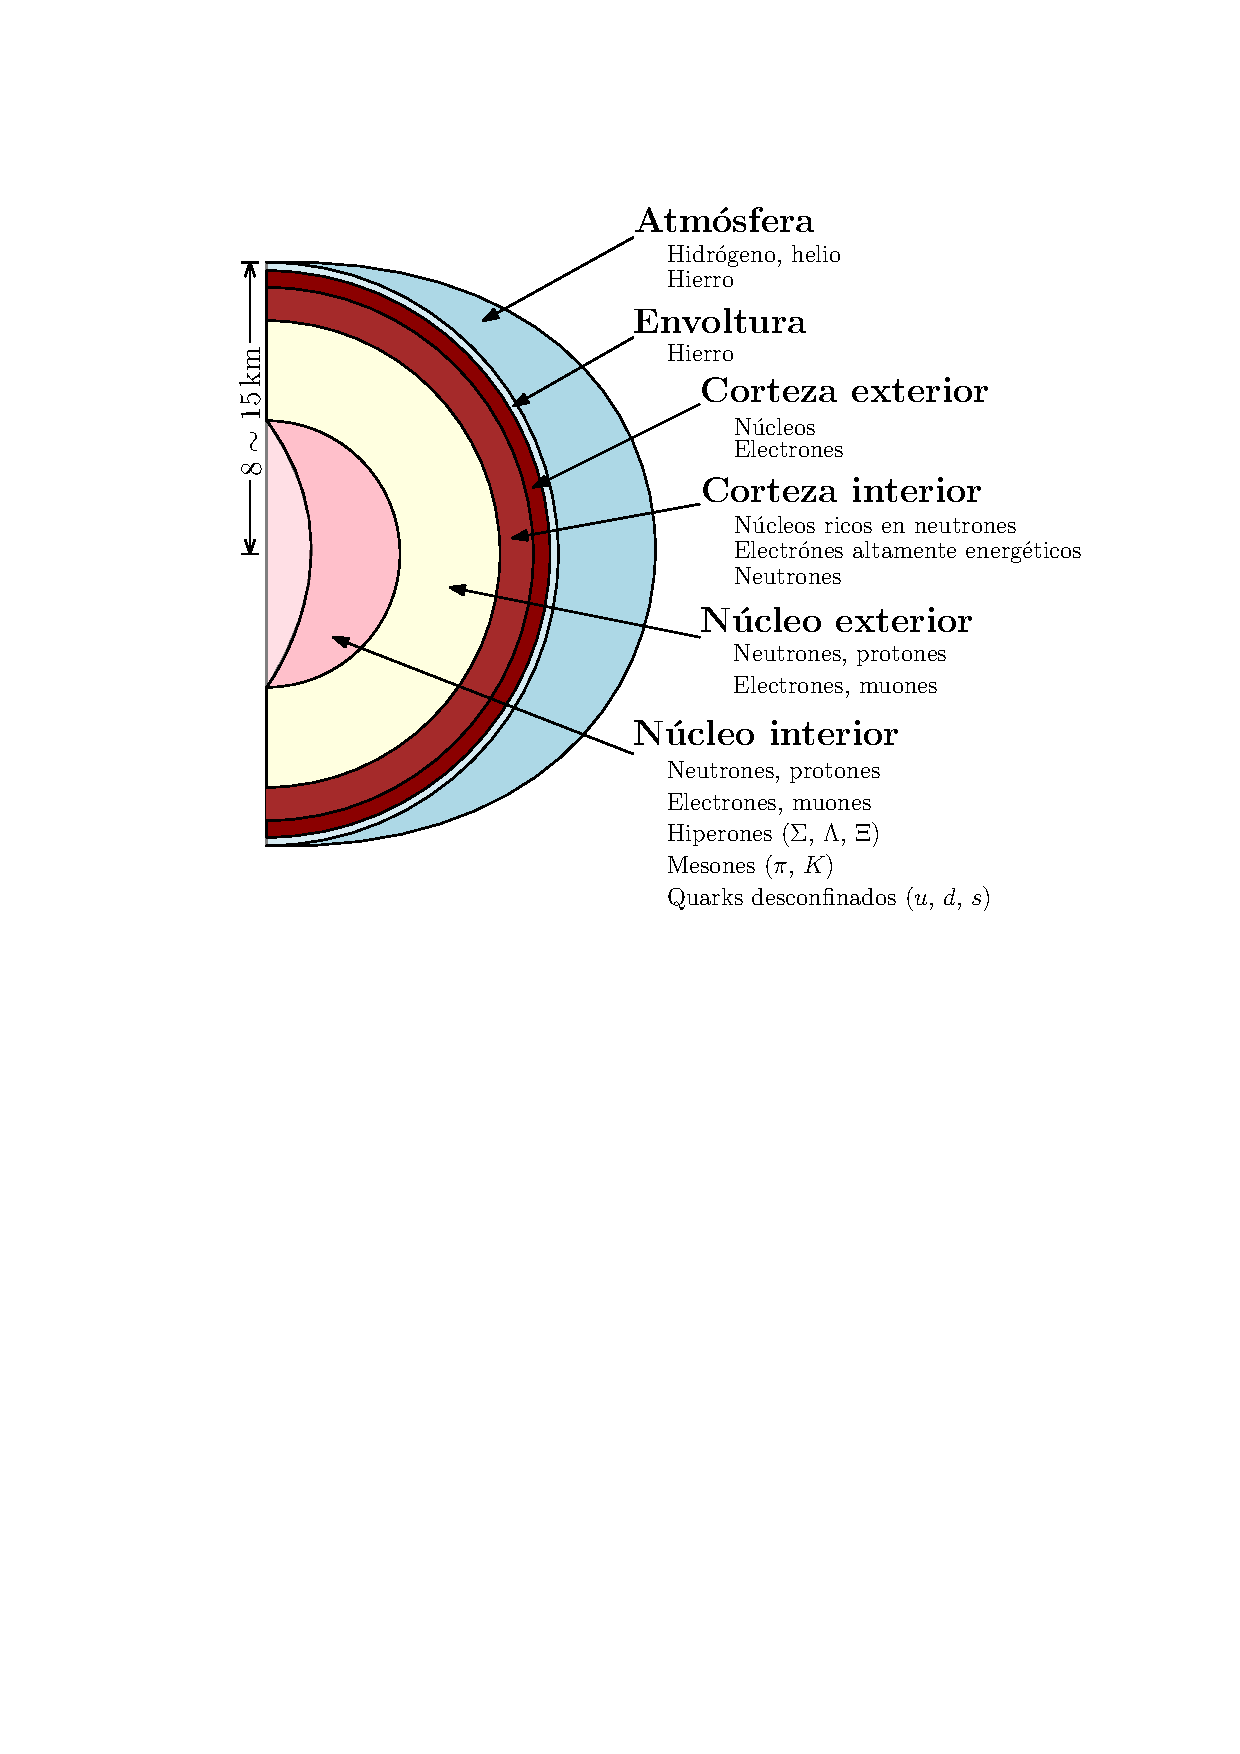
\includegraphics[width=300pt]{figures/neutronstar.pdf}
    \caption{Composición de una estrella de neutrones.\protect\footnotemark}
    \label{NSC}
\end{figure}
\footnotetext{Original: Figura 1 de \cite{Weber2012}}


El \emph{núcleo} comprende regiones en las que la densidad alcanza $\rho_0$ y contiene la mayor fracción de la masa estelar. Está subdividido un dos: el \emph{núcleo exterior}, con densidad $\num{0.5}\rho_0\lesssim\rho\lesssim 2\rho_0$  cuya composición se conoce bien cualitativamente \cite{Haensel2007NeutronStructure}: es un superfluido de neutrones y protones, con presencia de electrones y muones altamente degenerados. Del \emph{núcleo interior}, por el contrario, no se conoce su composición. Se ha sugerido la presencia de hiperones, piones, kaones e incluso quarks desconfinados (consultar las revisiones \cite{Potekhin,Lattimer2004} y referencias allí citadas).



La gran variedad de fases que se encuentran a medida de que la densidad aumenta en el interior de las estrellas de neutrones están ilustradas en la Figura \ref{NSS}. 

\begin{figure}[H]
    \centering
    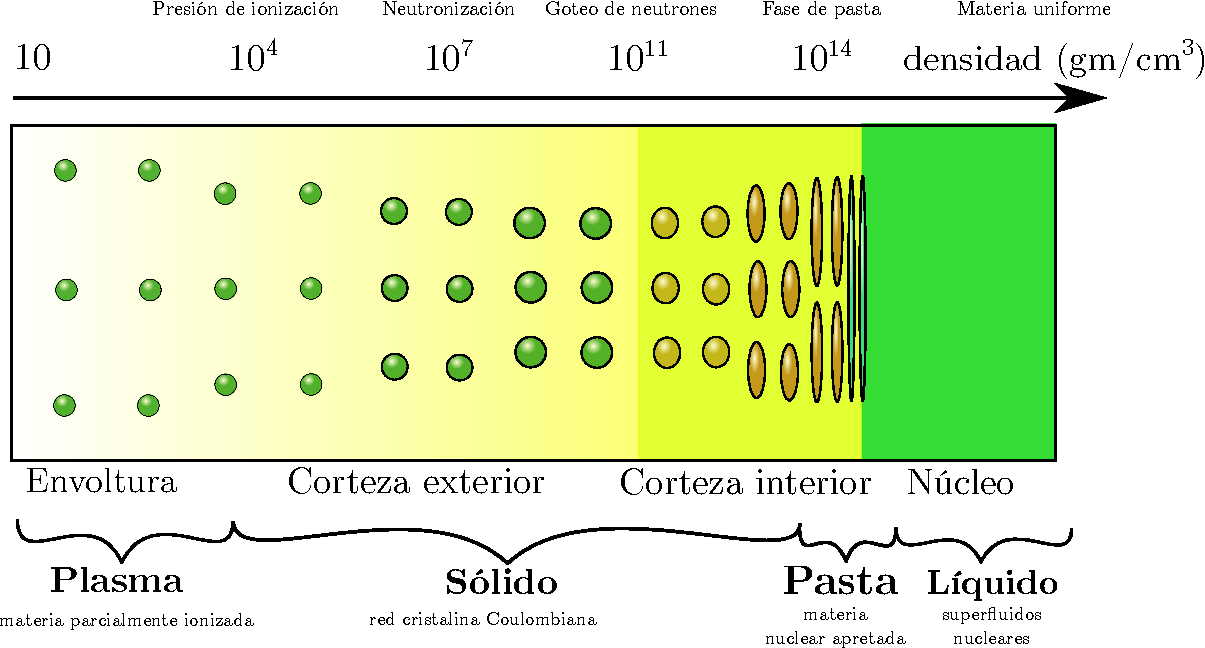
\includegraphics[width=420pt]{figures/Density.pdf}
    \caption[Estructura interna de una estrella de neutrones]{Estructura interna de una estrella de neutrones.\protect\footnotemark}
    \label{NSS}
\end{figure}
\footnotetext{Original: Figura 4 de \cite{Chamel2008}}   

\section{Ecuación de estado}

Como se mencionó en la Sección \ref{CR}, la ecuación de estado de la materia es necesaria para resolver las ecuaciones de TOV. Ésta se determina predominantemente de la interacción nuclear fuerte entre los constituyentes elementales de la materia y debido a que estas interacciones no son bien entendidas en materia a densidades superiores a la densidad de saturación nuclear $\rho_0$, la ecuación de estado de las estrellas de neutrones sigue siendo un misterio.

La mayoría de modelos de ecuaciones de estado se pueden agrupar en tres categorías: modelos de potencial no relativista, modelos de teoría de campos relativista y modelos de Dirac-Brueckner-Hartree-Fock relativistas. A continuación se presentarán algunos detalles de cada uno de estos enfoques.

\subsection{Modelos de potencial no relativista}
\subsection{Modelos de teoría de campos relativista}
\subsection{Modelos de Dirac-Brueckner-Hartree-Fock}
%\chapter{Solución numérica a las ecuaciones de TOV}

\chapter{Resultados}

Con el fin de determinar si los modelos de estrellas de neutrones obtenidos con las ecuaciones de estado de la materia densa disponibles en la literatura son físicamente viables, se resolvieron las ecuaciones de TOV \eqref{dmtov},\eqref{dptov} y \eqref{dnutov} para un amplio rango de densidades centrales y se evaluaron las condiciones C1-C11 presentadas en la Sección \ref{phyacep}.

En la siguiente sección se describirá el proceso de verificación detalladamente para la EOS ENG \cite{Engvik1994}, dado que predice una masa máxima $M_{\text{TOV}}$ superior a la masa del pulsar MSP J0740+6620 \cite{Cromartie2019} y además satisface los límites más conservadores impuestos por la primera observación de ondas gravitacionales por la fusión de dos estrellas de neutrones GW170817 y su contraparte electromagnética \cite{Rezzolla2017,Radice2018,Ruiz2018,Shibata2019}. Después se presentarán los resultados consolidados para un conjunto representativo de 37 EOSs (incluyendo ENG) basados en la elección de EOSs presente en la revisión \cite{Ozel2016}.

\section{Un caso particular: la ecuación de estado ENG}

ENG es una EOS para materia compuesta de neutrones, protones, electrones y muones asimétrica (con fracciones de protones distintas a $1/2$) que usa un enfoque miscroscópico (de acuerdo a la clasificación presentada en la Sección \ref{EOS}) basada en el método de Dirac-Brueckener-Hartree-Fock. 

Los requisitos mínimos de consistencia física que una ecuación de estado debe cumplir son la condición de energía dominante (C6) y la condición de causalidad (C7). Estas condiciones dependen enteramente de la construcción de la ecuación de estado y pueden ser verificadas sin necesidad de resolver las ecuaciones de TOV. En las Figuras \ref{DECeng} y \ref{SSCeng} se verificó que la EOS ENG cumple las condiciones C6 y C7.

\begin{figure}[H]
   \begin{minipage}[b]{.48\textwidth}
        \centering
        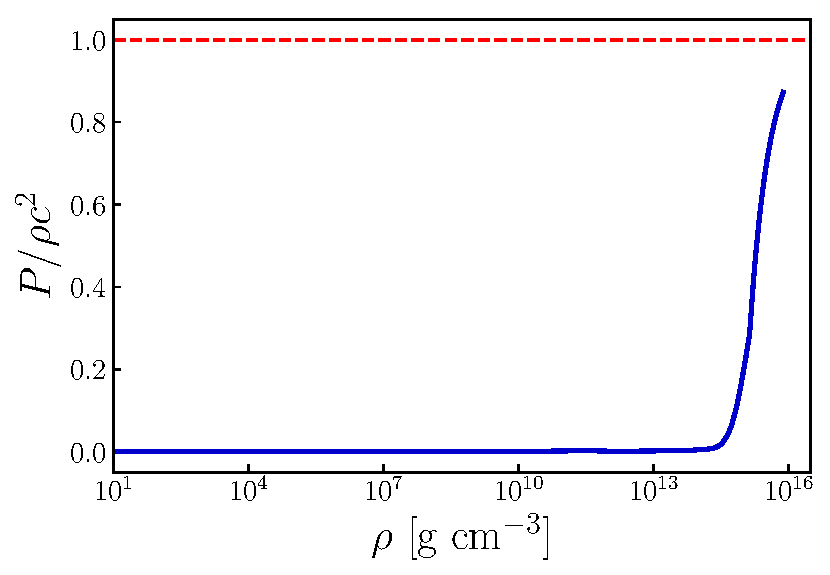
\includegraphics[width=1\textwidth]{figures/ECeng.pdf}
        \caption{Verificación de C6 para la EOS ENG. La línea roja punteada indica la igualdad $P=\rho c^2$. Se aprecia que $P/\rho c^2 \leq 1$, por lo que esta ecuación de estado cumple C6.}
        \label{DECeng}
    \end{minipage}
    \quad
    \begin{minipage}[b]{.48\textwidth}
        \centering
        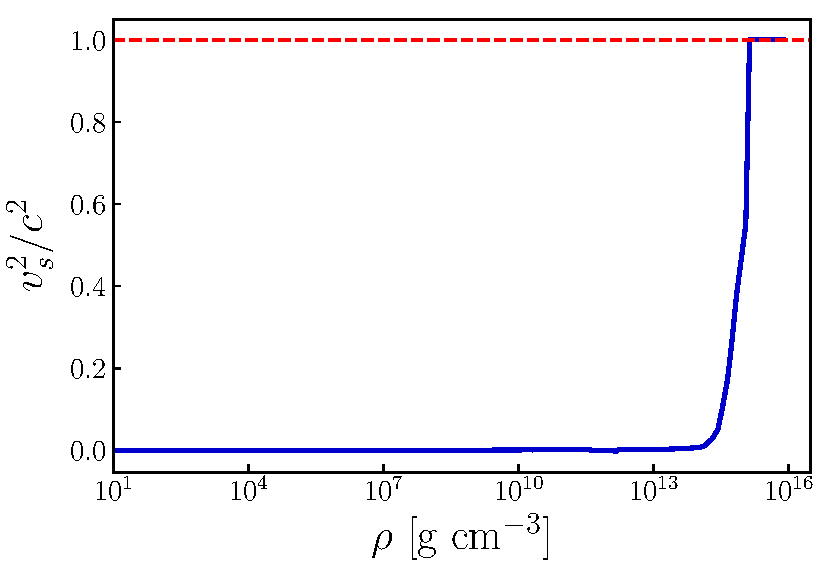
\includegraphics[width=1\textwidth]{figures/SSeng.pdf}
        \caption{Verificación de C7 para la EOS ENG. La línea roja punteada representa $v_s=c$. Se aprecia que $v_s^2/c^2 \leq 1$, por lo que esta ecuación de estado cumple C7.}
        \label{SSCeng}
    \end{minipage}
\end{figure}



\begin{figure}[H]
    \centering
    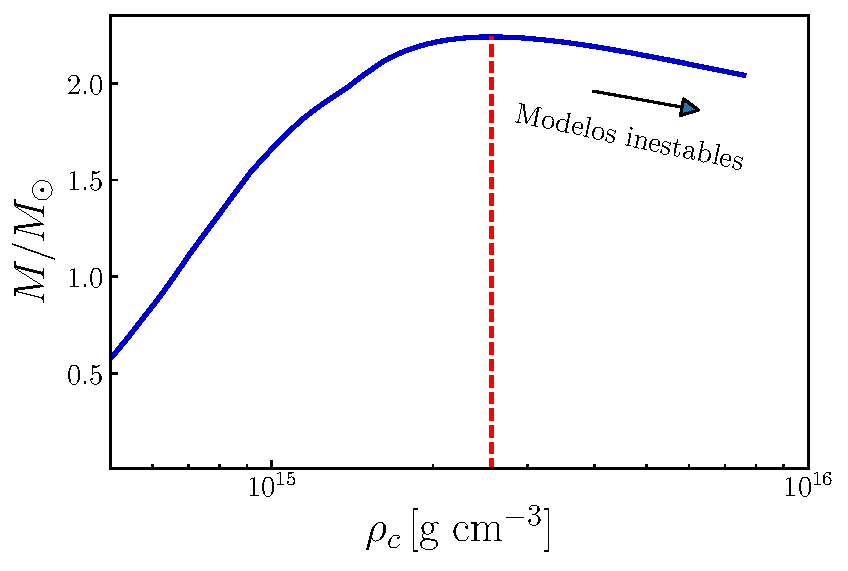
\includegraphics[width=0.7\linewidth]{figures/Mrhorel_eng.pdf}
    \caption{Identificando los modelos que no satisfacen C10. La masa máxima para esta ecuación de estado fue $M_{max}=2.241\,M_{\odot}$ alcanzada con la densidad central $\rho_c=2.5704 \times 10^{15}$ (línea roja punteada), así que modelos con $\rho_c \geq 2.5704 \times 10^{15}$ serán inestables ante pulsaciones radiales. }
    \label{mrhoeng}
\end{figure}

Tras confirmar que la ecuación de estado cumple C6 y C7, se procede a solucionar las ecuaciones de TOV para un conjunto de densidades centrales (valores iniciales) que típicamente va desde $\rho_c=\rho_0 \sim 10^{14} \text{g cm}^{-3}$ hasta la máxima densidad disponible en la ecuación de estado. Como las soluciones cumplen las condiciones de acoplamiento (C2) por construcción (como es descrito en el Apéndice \ref{NumSol}), se usa la condición C10 para restringir los modelos a analizar: sólo se considerarán modelos con densidades centrales tales que $\frac { \partial M \left( \rho _ { c } \right) } { \partial \rho _ { c } } > 0$. Esta derivada es nula para la configuración con masa máxima y se presenta un cambio del signo de la derivada de positiva a negativa, la densidad central para la que esto ocurre indica el inicio de las configuraciones inestables (ver Figura \ref{mrhoeng}).

Para continuar con el análisis de la estabilidad de los modelos que satisfacen C10 se halló la primera y segunda derivada respecto a la coordenada radial $r$ de $\rho$ y $P$ numéricamente (los detalles de cómo se obtuvo las derivadas numéricamente se encuentran en la Sección \ref{NumDer} del Apéndice \ref{NumSol}) con el objetivo de verificar las condiciones C9 y C11.  

Haciendo un análisis gráfico de $\dv{P(r)}{r} $ (ver Figura \ref{CrackStabilityeng}) se determinó que todos los modelos que satisfacen C10 también satisfacen C9. 
 

\begin{figure}[H]
    \centering
    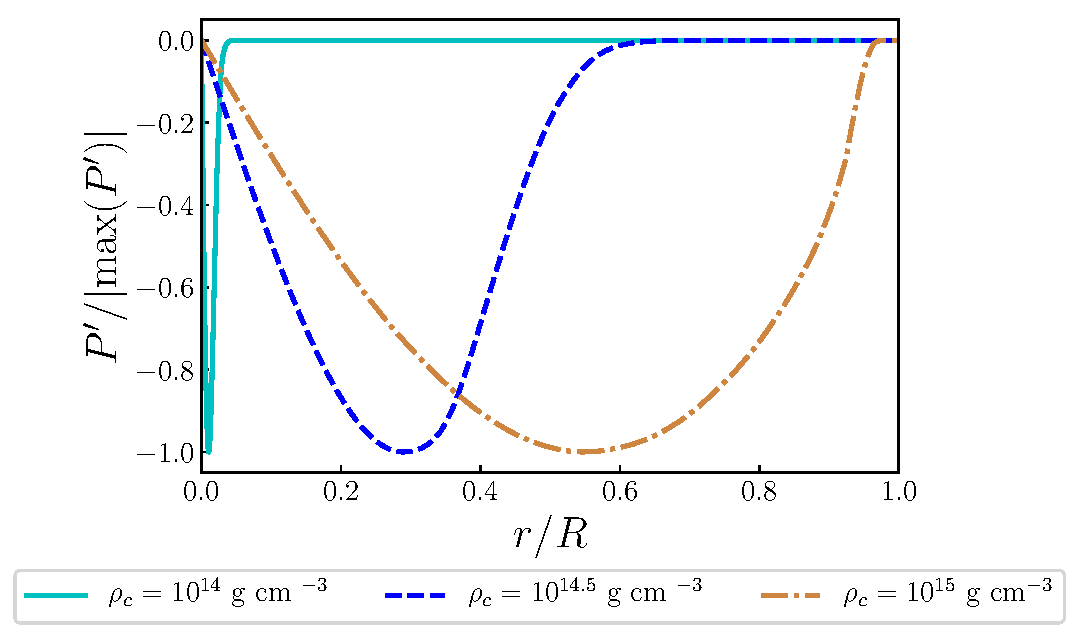
\includegraphics[width=0.93\linewidth]{figures/CrackStabilityeng.pdf}
    \caption{Verificación de C9. Se presentan los gradientes de presión de una muestra representativa de los modelos que cumplen con C10. Estos siempre son menores  iguales a cero  y por lo tanto los modelos considerados son estables ante cracking.}
    \label{CrackStabilityeng}
\end{figure}

Por otro lado, el análisis gráfico de $\dv[2]{\rho}{r}$ reveló que en todos los modelos hay una región en la cual no se cumple la condición C11 (ver Figura \ref{ConvecStabilityeng}). Al graficar $\dv[2]{\rho}{r}$ contra $\rho$ (ver Figura \ref{ConvecStabilityengCorrel}) se identifica que la zona que no cumple la condición C11 está acotada entre densidades cercanas a $\rho_{ND}\approx 4 \times 10^{11} $ y densidades cercanas $\rho_0$ (aŕea sombreada). Este rango de densidades concuerda con las encontradas en la corteza interior (ver Figura \ref{NSS}) y sugiere que la corteza interior hace que los modelos obtenidos con la EOS ENG sean inestables antes ante convección adiabática. 

\begin{figure}[H]
    \centering
    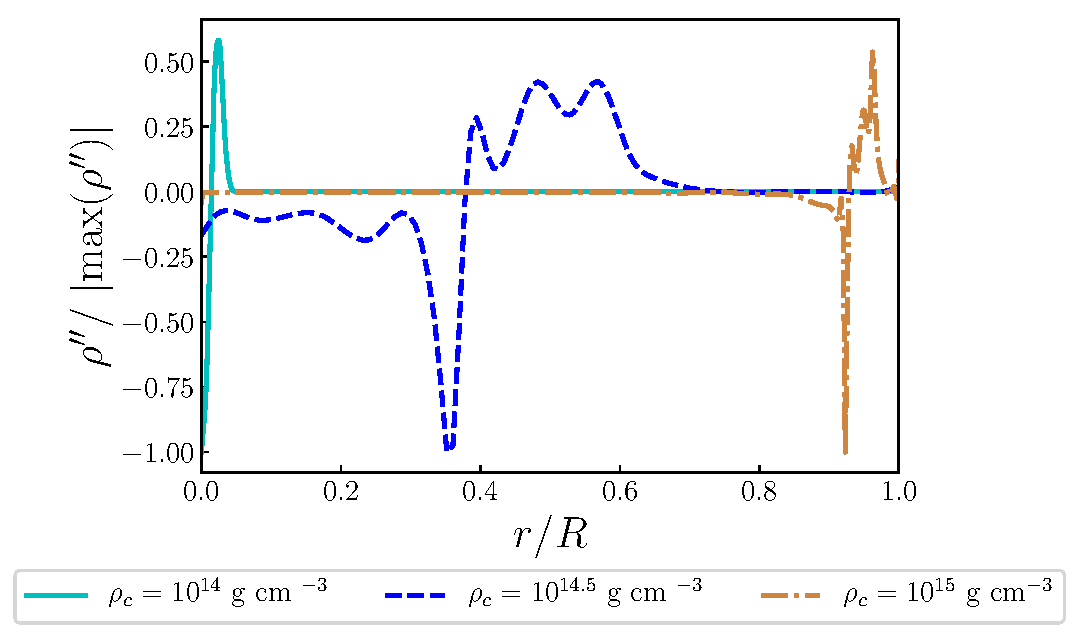
\includegraphics[width=0.93\linewidth]{figures/ConvecStabilityeng.pdf}
    \caption{Verificación de C11. Se presenta $\rho^{\prime\prime}(r)$ de una muestra representativa de los modelos que cumplen con C10. La condición no se cumple en toda la estrella para todos los modelos. }
    \label{ConvecStabilityeng}
\end{figure}
\begin{figure}[H]
    \centering
    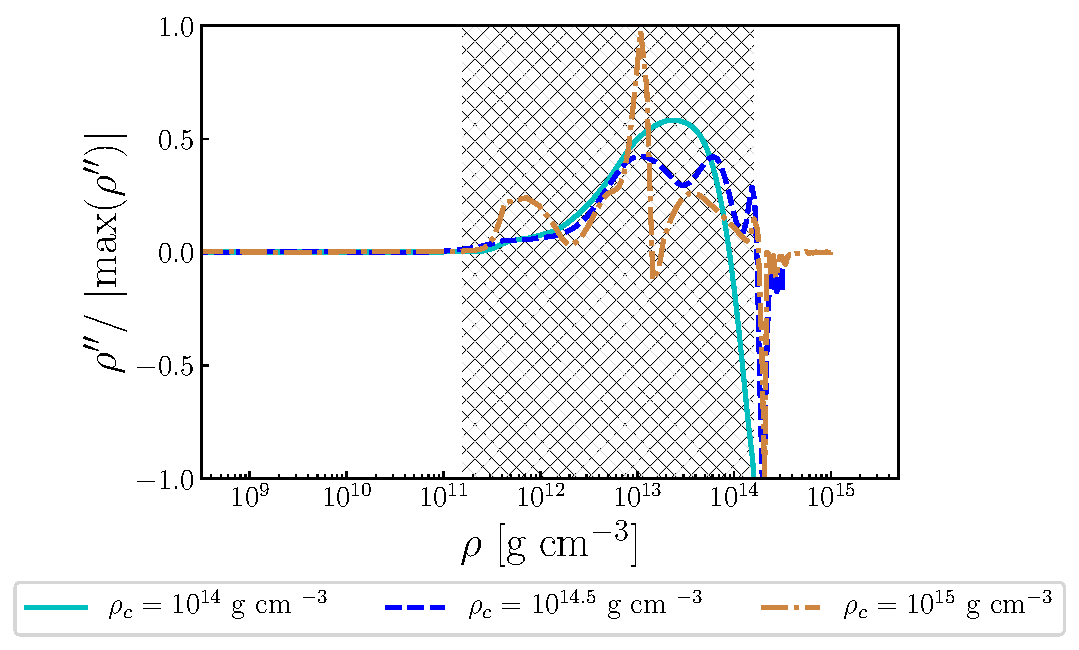
\includegraphics[width=0.93\linewidth]{figures/ConvecStabilityengCorrel.pdf}
    \caption{El gráfico $\rho^{\prime\prime}(\rho)$ permite identificar la ubicación de las inestabilidades: para todos los modelos se encuentran en el rango de densidades ($\rho_{ND},\rho_0$) (área sombreada), lo que indica que se trata de la corteza interior de la estrella.} 
    \label{ConvecStabilityengCorrel}
\end{figure}

Finalmente se verificó que los modelos considerados son consistentes con la condición C3 calculando el corrimiento al rojo como función de la coordenada radial \eqref{redshift} (ver Figura \ref{Redshifteng}). 

\begin{figure}[H]
    \centering
    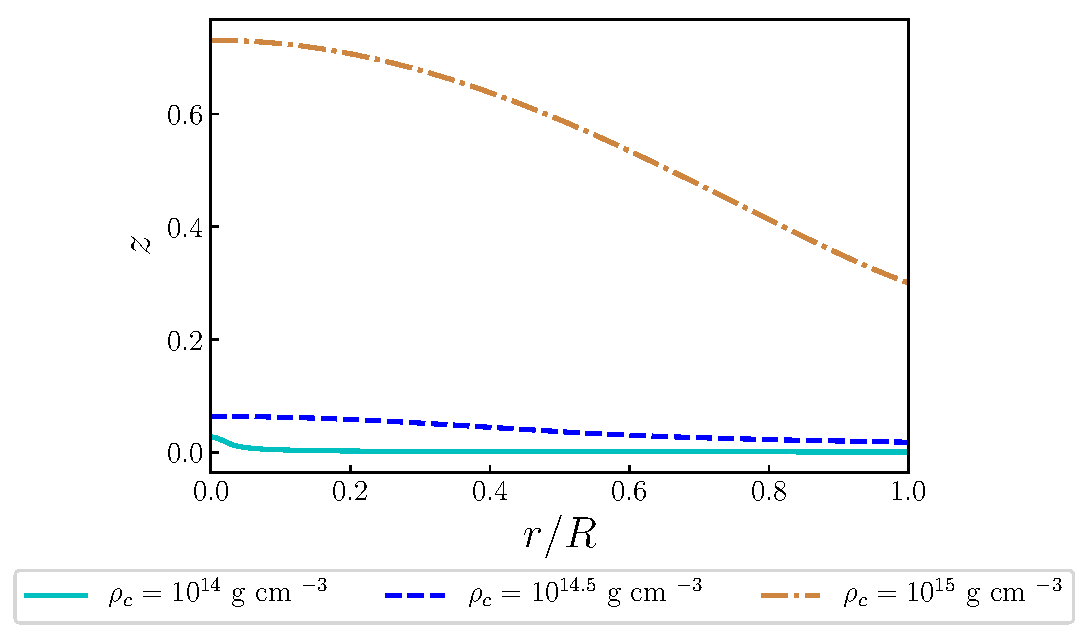
\includegraphics[width=0.93\linewidth]{figures/Redshifteng.pdf}
    \caption{Verificación de C3. Se graficó el corrimiento al rojo $z$ como una función de $r$. Se aprecia que $z$ decrece alcanzando un mínimo en el borde de la estrella para los modelos considerados, satisfaciendo C3.}
    \label{Redshifteng}
\end{figure}

\section{Consolidados}

Tras realizar un análisis análogo al presentado en la sección anterior para todo el conjunto de 37 EOSs, los resultados fueron sintetizados en la Tabla \ref{Consolidados} y pueden ser consultados en el notebook de Jupyter \href{https://nbviewer.jupyter.org/github/DavidRamosSal/stellar_structure/blob/master/RAnalysis.ipynb}{RAnalysis}. En primer lugar se encontró que todas las EOSs consideradas producen modelos estelares que son estables ante cracking. Se encontró que 31 de las 37 EOSs producen modelos estelares que presentan inestabilidades convectivas en la corteza interior (comportamiento descrito en la Figura \ref{ConvecStabilityengCorrel}).

Tres EOSs (H4-7) no pudieron ser evaluadas rigurosamente pues las tablas sólo contenían la parte más densa de la EOS ($\rho > 10^{14}$), presuntamente para ser acoplada posteriormente con una EOS para la corteza y por lo tanto no se pudo evaluar la estabilidad convectiva en esta región. Finalmente, para tres EOSs (SQM1-3) se encontró que los modelos producidos son inestables ante convección adiabática sólo cerca a la superficie. Como la región en la que se presentan las inestabilidades corresponde a un rango de densidades muy reducido cercano al borde  de la estrella, puede deberse a un error numérico.

Los valores de $M_{\text{max}}$ y el respectivo radio $R_{M_{\text{max}}}$ calculados para cada EOS son cercanos a los obtenidos en \cite{Read2009} para un conjunto similar de EOSs y representan por lo tanto otra forma de validar los cálculos. Sin embargo, como este trabajo está orientado al análisis de los perfiles de densidad y presión, no se procederá a calcular diferencias para estos parámetros entre las dos simulaciones. 

\begin{table}[H]
\caption{Resultados para las 37 EOSs consideradas. C3: corrimiento al rojo, C6: condición de energía dominante, C7: causalidad, C9: cracking, C11: movimientos convectivos. Se listan además el método teórico usado para obtener la EOS, los componentes que interactúan fuertemente (todos los modelos incluyen contribuciones leptónicas), la masa máxima $M_{\text{max}}$ y el respectivo radio $R_{M_{\text{max}}}$ para estrellas estáticas y la referencia a los trabajos originales.}
\label{Consolidados}
\begin{adjustbox}{max width=\textwidth}
\begin{tabular}{ccccccccccc}
\hline
\multirow{2}{*}{\textbf{EOS}} & \multirow{2}{*}{\textbf{Método}}           & \multirow{2}{*}{\textbf{Composición}} & \multirow{2}{*}{\begin{tabular}[c]{@{}c@{}}$\mathbf{M}_{\text{\textbf{max}}}$\\  $[\mathbf{M_{\odot}}]$\end{tabular}} & \multirow{2}{*}{\begin{tabular}[c]{@{}c@{}}$\mathbf{R}_{\mathbf{M}_{\text{\textbf{max}}}}$\\  $[$\textbf{km}$]$\end{tabular}} & \multirow{2}{*}{\textbf{C3}} & \multirow{2}{*}{\textbf{C6}} & \multirow{2}{*}{\textbf{C7}} & \multirow{2}{*}{\textbf{C9}} & \multirow{2}{*}{\textbf{C11}} & \multirow{2}{*}{\textbf{Referencia}}          \\
                     &                                   &                              &                                                                                            &                                                                                           &                     &                     &                     &                     &                      &                                      \\ \hline \addlinespace
ALF1                 & \multirow{4}{*}{Mixto}            & \multirow{4}{*}{$n,p,q$}     & 1.496                                                                                      & 9.221                                                                                     & \checkmark          & \checkmark          & \checkmark          & \checkmark          & \Cross               & \multirow{4}{*}{\cite{Alford2005}}   \\
ALF2                 &                                   &                              & 2.087                                                                                      & 11.962                                                                                    & \checkmark          & \checkmark          & \checkmark          & \checkmark          & \Cross               &                                      \\
ALF3                 &                                   &                              & 1.473                                                                                      & 9.514                                                                                     & \checkmark          & \checkmark          & \checkmark          & \checkmark          & \Cross               &                                      \\
ALF4                 &                                   &                              & 1.943                                                                                      & 10.892                                                                                    & \checkmark          & \checkmark          & \checkmark          & \checkmark          & \Cross               &                                      \\ \addlinespace
AP1                  & \multirow{4}{*}{Variacional}      & \multirow{4}{*}{$n,p$}       & 1.684                                                                                      & 8.292                                                                                     & \checkmark          & \checkmark          & \checkmark          & \checkmark          & \Cross               & \multirow{4}{*}{\cite{Akmal1998}}    \\
AP2                  &                                   &                              & 1.809                                                                                      & 8.746                                                                                     & \checkmark          & \checkmark          & \Cross              & \checkmark          & \Cross               &                                      \\
AP3                  &                                   &                              & 2.391                                                                                      & 10.765                                                                                    & \checkmark          & \Cross              & \Cross              & \checkmark          & \Cross               &                                      \\
AP4                  &                                   &                              & 2.214                                                                                      & 10.004                                                                                    & \checkmark          & \Cross              & \Cross              & \checkmark          & \Cross               &                                      \\ \addlinespace
BBB2                 & Brueckener HF                     & $n,p$                        & 1.920                                                                                      & 9.515                                                                                     & \checkmark          & \checkmark          & \checkmark          & \checkmark          & \Cross               & \cite{Lombardo2004}                  \\ \addlinespace
BGN1H1               & Potencial efectivo                & $n,p,H$                      & 1.630                                                                                      & 9.325                                                                                     & \checkmark          & \checkmark          & \checkmark          & \checkmark          & \Cross               & \cite{Balberg1997}                   \\ \addlinespace
BPAL12               & Brueckener HF                     & $n,p$                        & 1.455                                                                                      & 9.015                                                                                     & \checkmark          & \checkmark          & \checkmark          & \checkmark          & \Cross               & \cite{Zuo1999}                       \\ \addlinespace
BSK19                & \multirow{3}{*}{DFT}              & \multirow{3}{*}{$n,p$}       & 1.861                                                                                      & 9.110                                                                                     & \checkmark          & \Cross              & \Cross              & \checkmark          & \Cross               & \multirow{3}{*}{\cite{Potekhin2013}} \\
BSK20                &                                   &                              & 2.165                                                                                      & 10.173                                                                                    & \checkmark          & \Cross              & \Cross              & \checkmark          & \Cross               &                                      \\
BSK21                &                                   &                              & 2.274                                                                                      & 11.038                                                                                    & \checkmark          & \Cross              & \Cross              & \checkmark          & \Cross               &                                      \\ \addlinespace
ENG                  & Brueckener HF                     & $n,p$                        & 2.241                                                                                      & 10.425                                                                                    & \checkmark          & \checkmark          & \checkmark          & \checkmark          & \Cross               & \cite{Engvik1994}                    \\ \addlinespace
FPS                  & Variacional                       & $n,p$                        & 1.800                                                                                      & 9.279                                                                                     & \checkmark          & \checkmark          & \checkmark          & \checkmark          & \Cross               & \cite{Friedman1981}                  \\ \addlinespace
GNH3                 & Teoría de campos                  & $n,p,H,\Delta$               & 1.965                                                                                      & 11.372                                                                                    & \checkmark          & \checkmark          & \checkmark          & \checkmark          & \Cross               & \cite{Glendenning1985}               \\ \addlinespace
H1                   & \multirow{6}{*}{Teoría de campos} & \multirow{6}{*}{$n,p,H$}     & 1.556                                                                                      & 10.968                                                                                    & \checkmark          & \checkmark          & \checkmark          & \checkmark          & \Cross               & \multirow{6}{*}{\cite{Lackey2006}}   \\
H2                   &                                   &                              & 1.668                                                                                      & 11.516                                                                                    & \checkmark          & \checkmark          & \checkmark          & \checkmark          & \Cross               &                                      \\
H3                   &                                   &                              & 1.790                                                                                      & 11.863                                                                                    & \checkmark          & \checkmark          & \checkmark          & \checkmark          & \Cross               &                                      \\
H4                   &                                   &                              & 2.032                                                                                      & 11.467                                                                                    & \checkmark          & \checkmark          & \checkmark          & \checkmark          & -           &                                      \\
H5                   &                                   &                              & 1.726                                                                                      & 10.930                                                                                    & \checkmark          & \checkmark          & \checkmark          & \checkmark          &  -           &                                      \\
H7                   &                                   &                              & 1.683                                                                                      & 10.474                                                                                    & \checkmark          & \checkmark          & \checkmark          & \checkmark          & -           &                                      \\ \addlinespace
MPA1                 & Brueckener HF                     & $n,p$                        & 2.462                                                                                      & 11.301                                                                                    & \checkmark          & \checkmark          & \checkmark          & \checkmark          & \Cross               & \cite{Muther1987}                    \\ \addlinespace
MS1                  & \multirow{2}{*}{Teoría de campos} & \multirow{2}{*}{$n,p$}       & 2.770                                                                                      & 13.346                                                                                    & \checkmark          & \checkmark          & \checkmark          & \checkmark          & \Cross               & \multirow{2}{*}{\cite{Muller1996}}   \\
MS1b                 &                                   &                              & 2.778                                                                                      & 13.301                                                                                    & \checkmark          & \checkmark          & \checkmark          & \checkmark          & \Cross               &                                      \\ \addlinespace
NL3                  & Teoría de campos                  & $n,p,\sigma,\omega,\rho$     & 2.806                                                                                      & 13.427                                                                                    & \checkmark          & \checkmark          & \checkmark          & \checkmark          & \Cross               & \cite{Lalazissis1997}                \\ \addlinespace \hline \addlinespace
\multicolumn{1}{l}{} & \multicolumn{1}{l}{}              & \multicolumn{1}{l}{}         & \multicolumn{1}{l}{}                                                                       & \multicolumn{1}{l}{}                                                                      & \multicolumn{1}{l}{} & \multicolumn{1}{l}{} & \multicolumn{4}{l}{\small{(Continúa en la siguiente página)}} 
\end{tabular}
\end{adjustbox}
\end{table}


% Please add the following required packages to your document preamble:
% \usepackage{multirow}
\begin{table}[H]
\renewcommand\thetable{3.1 (continuación)}
\caption{}
\begin{adjustbox}{max width=\textwidth}
\begin{tabular}{ccccccccccc}
\hline
\multirow{2}{*}{\textbf{EOS}} & \multirow{2}{*}{\textbf{Método}}           & \multirow{2}{*}{\textbf{Composición}} & \multirow{2}{*}{\begin{tabular}[c]{@{}c@{}}$\mathbf{M}_{\text{\textbf{max}}}$\\  $[\mathbf{M_{\odot}}]$\end{tabular}} & \multirow{2}{*}{\begin{tabular}[c]{@{}c@{}}$\mathbf{R}_{\mathbf{M}_{\text{\textbf{max}}}}$\\  $[$\textbf{km}$]$\end{tabular}} & \multirow{2}{*}{\textbf{C3}} & \multirow{2}{*}{\textbf{C6}} & \multirow{2}{*}{\textbf{C7}} & \multirow{2}{*}{\textbf{C9}} & \multirow{2}{*}{\textbf{C11}} & \multirow{2}{*}{\textbf{Referencia}}          \\
                     &                                   &                              &                                                                                            &                                                                                           &                     &                     &                     &                     &                      &                                      \\ \hline \addlinespace
PAL6                 & Mixto                             & $n,p$                        & 1.478                                                                                      & 9.258                                                                                     & \checkmark          & \checkmark          & \checkmark          & \checkmark          & \Cross               & \cite{Prakash1988}                   \\ \addlinespace
PCL2                 & Teoría de campos                  & $n,p,H,q$                    & 1.483                                                                                      & 10.116                                                                                    & \checkmark          & \checkmark          & \checkmark          & \checkmark          & \Cross               & \cite{Prakash1995}                   \\ \addlinespace
PS                   & Teoría de campos                  & $n,\pi^0$                    & 1.755                                                                                      & 11.372                                                                                    & \checkmark          & \checkmark          & \checkmark          & \checkmark          & \Cross               & \cite{Pandharipande1975}             \\ \addlinespace
SLy                  & Mixto                             & $n,p$                        & 2.050                                                                                      & 9.977                                                                                     & \checkmark          & \checkmark          & \Cross              & \checkmark          & \Cross               & \cite{Douchin2001}                   \\ \addlinespace
SQM1                 & \multirow{3}{*}{Teoría de campos} & \multirow{3}{*}{$q$}         & 1.532                                                                                      & 8.315                                                                                     & \checkmark          & \checkmark          & \checkmark          & \checkmark          & -*                    & \multirow{3}{*}{\cite{Prakash1995}}  \\
SQM2                 &                                   &                              & 1.737                                                                                      & 9.638                                                                                     & \checkmark          & \checkmark          & \checkmark          & \checkmark          & -*                    &                                      \\
SQM3                 &                                   &                              & 1.977                                                                                      & 10.814                                                                                    & \checkmark          & \checkmark          & \checkmark          & \checkmark          & -*                    &                                      \\ \addlinespace
WFF1                 & \multirow{3}{*}{Variacional}      & \multirow{3}{*}{$n,p$}       & 2.134                                                                                      & 9.413                                                                                     & \checkmark          & \checkmark          & \Cross              & \checkmark          & \Cross               & \multirow{3}{*}{\cite{Wiringa1988}}  \\
WFF2                 &                                   &                              & 2.199                                                                                      & 9.825                                                                                     & \checkmark          & \checkmark          & \Cross              & \checkmark          & \Cross               &                                      \\
WFF3                 &                                   &                              & 1.845                                                                                      & 9.516                                                                                     & \checkmark          & \checkmark          & \checkmark          & \checkmark          & \Cross               &                                      \\ \addlinespace \hline \addlinespace
\multicolumn{3}{l}{\small{*Resultados con problemas en la frontera}}                                            & \multicolumn{1}{l}{}                                                                       & \multicolumn{1}{l}{}                                                                      & \multicolumn{1}{l}{} & \multicolumn{1}{l}{} & \multicolumn{1}{l}{} & \multicolumn{1}{l}{} & \multicolumn{1}{l}{} & \multicolumn{1}{l}{}             
\end{tabular}
\end{adjustbox}
\end{table}

\section{Discusión}

A continuación se presentará una discusión sobre los resultados encontrados para las condiciones de aceptabilidad evaluada.

\emph{C3}. A pesar de que el valor del corrimiento al rojo gravitacional $z$ en la superficie sea muy sensible a la EOS utilizada (por estar relacionado con la masa y el radio de la estrella), se encontró que el comportamiento de $z$ como función de la coordenada $r$ no varía entre las EOSs: decrece monótonamente del centro al borde de la esfera satisfaciendo la condición de aceptabilidad y aumenta globalmente con la densidad central (Figura \ref{Redshifteng}).

\emph{C6} y \emph{C7}. Tras encontrar que EOSs usadas ampliamente en aplicaciones no cumplen estas condiciones surge la pregunta: ¿puede una EOS físicamente correcta violar C6 y C7? De acuerdo a \cite{Haensel2007} existen ejemplos de modelos que a pesar de no cumplir C6 y C7 siguen siendo siendo causales e invariantes ante transformaciones de Lorentz. Sin embargo, el hecho de que los modelos que no cumplen estas condiciones están basados en esquemas de muchos cuerpos no relativistas sugiere que los modelos son artificiales pues este tipo de comportamientos no se presenta en esquemas relativistas. Además, se encontró que todas las ecuaciones que no cumplen C6 tampoco cumplen C7, mientras que lo opuesto no se cumple, esto sugiere que otras características aparte de la rigidez de la EOS pueden resultar en violaciones a C7. Por otro lado se ha sugerido que la condición C7 se debe cumplir sólo a densidades realizables en las estrellas de neutrones \cite{Douchin2001}, esto es, a densidades menores a la densidad para la que se obtiene la masa máxima. Si esto es correcto, algunas de las EOS que cumplen C6 pero no C7 seguirían siendo físicamente aceptables, pero no se intentará resolver ese problema en este trabajo.

\emph{C9}. A pesar de que ha sido sugerido que el cracking puede ocurrir en modelos isótropos \cite{Hernandez2018,Gonzalez2014}, se encontró que todos los modelos son estables ante cracking, este resultado era esperado por tratarse de soluciones de fluido perfecto y se ha obtenido para otras soluciones exactas interiores isótropas como la Tolman VI \cite{Herrera1992}.

\emph{C11}. Los resultados indican que según el criterio C11 la corteza interior de las estrellas de neutrones es inestable ante convección, para todas las EOSs. Previamente en \cite{Miralles1997} se mostró que en estrellas débilmente magnetizadas, la envoltura de la estrella de neutrones puede ser inestable ante convección. Sin embargo, nada se ha reportado acerca de la estabilidad de la corteza interior. Es sabido \cite{Haensel2007} que las transiciones de fase primer orden que ocurren en la interfaz corteza-núcleo producen discontinuidades en el perfil de densidad, esto es observado en los resultados (pico en regiones con densidades cercanas a $\rho_0$ en la Figura \ref{ConvecStabilityengCorrel}) y puede tener algo que ver con la existencia de la inestabilidad en regiones que se acercan a estas densidades. Este resultado puede ser importante debido a que se ha discutido la posibilidad de que los superfluidos presentes en la corteza interior generen corrientes de convección hacia las regiones más externas de la estrella. 

\chapter*{Conclusiones}
\addcontentsline{toc}{chapter}{Conclusiones}
%El comportamiento de la materia en las estrellas de neutrones 
%Al día de hoy nuestra comprensión de las leyes de la física a densidades altas sigue siendo pobre. 
%La EOS de la materia en el interior de las estrellas de neutrones sigue siendo al día de hoy un misterio. Además de su importancia práctica en simulaciones de diferentes eventos astrofísicos,
\noindent Más allá de su utilidad práctica en simulaciones de supernovas y otros eventos astronómicos, la importancia de determinar la EOS de la materia al interior de las estrellas de neutrones reside en que nos permite entender el comportamiento de las leyes de la física a densidades que no son realizables experimentalmente en la tierra. La existencia de múltiples candidatos sólo refleja nuestra inhabilidad para aplicar nuestro conocimiento de física nuclear en condiciones tan extremas como las encontradas en las estrellas de neutrones. El objetivo de este trabajo fue aplicar criterios de aceptabilidad física a los modelos de estrellas de neutrones estáticas obtenidos con diferentes EOSs con el fin de identificar candidatos que produzcan modelos que no sean realistas. 

Tras una breve discusión sobre los aspectos generales de las estrellas de neutrones, se presentó una deducción de las ecuaciones de estructura estelar tanto en la teoría Newtoniana como en la relativista y se explicó cómo brindando una EOS es posible construir modelos estelares. Las condiciones de aceptabilidad fueron presentadas y aplicadas a un conjunto de 37 EOSs que varían ampliamente en composición y rigidez. En lo que concierne a las condiciones C1-10 los resultados obtenidos en este trabajo habían sido presentados en los artículos originales y parcialmente en otros trabajos \cite{Ozel2016,Read2009}, excepto para la condición C4: el problema encontrado al aplicar los criterios existentes para restringir el valor del índice adiabático al interior de la estrella no ha sido reportado. 

Los resultados obtenidos para la condición C11 fueron inesperados: la corteza interior de los modelos obtenidos con todas las EOSs consideradas es inestable ante movimientos convectivos adiabáticos. La posibilidad de que la corteza interna presente inestabilidades convectivas no ha sido reportada antes y debido a la complejidad de los modelos físicos desarrollados para describir fenómenos como la superfluidez y cambios de fase que ocurren esta región, es difícil identificar posibles causas. Este resultado puede ser importante dado que se cree que existe convección de superfluido de esta región hacia otras \cite{Haensel2007}. 

Respecto a la confiabilidad de los resultados obtenidos cabe resaltar que la rutina numérica reproduce diferentes soluciones exactas de fluido perfecto con gran precisión y que los problemas de usar diferencias finitas para calcular derivadas numéricas fueron superados con la ayuda de un spline con un factor de suavizamiento. Así mismo, los resultados de la masas máximas y los respectivos radios para cada EOS concuerdan con lo presentado en otros trabajos.

Una de las inquietudes que puede surgir al aplicar el criterio C11 a modelos de estrellas de neutrones es que éste es Newtoniano en esencia (es una consecuencia directa del principio de Arquímedes) y su validez en el contexto de la relatividad general no está asegurada. Sin embargo, como ha sido argumentado para criterios de estabilidad ante convección Newtonianos más generales, a diferencia de las pulsaciones que son fenómenos globales, la inestabilidad ante convección es un fenómeno local que está gobernado enteramente por los valores locales de las variables termodinámicas \cite{Thorne1966}.    

La metodología de este trabajo es análoga a la presentada en \cite{Delgaty1998} para soluciones exactas y, en vista del resultado obtenido para la estabilidad convectiva, complementa el uso de observaciones para restringir modelos de EOSs de una manera fundamental, puesto que permite identificar partes específicas del conocimiento actual en las que es posible no se haya explorado todo el rango de posibilidades físicas.

Finalmente, se espera extender el trabajo realizado para incluir más EOSs, incluyendo modernas EOSs de "alta precisión" que permitirían reducir los errores numéricos inherentes a la interpolación y analizar mejor la estabilidad de la corteza interior.



% This displays the bibliography for all cited external documents. All references have to be defined in the file references.bib and can then be cited from within this document.
\bibliographystyle{hieeetr}

\bibliography{references}\TODO{Chequear que los links estén correctos.}


% This creates an appendix chapter, comment if not needed.

\appendix

\chapter{Curvatura de un espacio-tiempo estático con simetría esférica}\label{curvature}

La métrica de un espacio-tiempo estático con simetría esférica está dada por
\begin{equation}
    \bm{g}=-e^{2 a(r)} \dd{t} \otimes \dd{t}+e^{2 b(r)} \dd{r} \otimes \dd{r} +r^{2}\left(\dd{\theta} \otimes \dd{\theta}+\operatorname{sen}^{2} \theta \dd{\varphi} \otimes \dd{\varphi}\right),
\end{equation}
el tensor de curvatura de Riemann correspondiente a esta métrica puede ser calculado de manera simple haciendo uso del cálculo de Cartan. 

En el cálculo de Cartan se hace uso del hecho de que es posible escoger como base del espacio cotangente $T^{*}_p$ en un punto $p$ de la variedad, una base $\omega^{\alpha}$ diferente a la base coordenada $\dd{x^\alpha}$. Esta base se escoge de modo tal que la métrica pueda ser escrita como 
\begin{equation}
    \bm{g}=\tensor{\eta}{_\alpha_\beta} \omega^{\alpha} \otimes \omega^{\beta},
\end{equation}
donde $\tensor{\eta}{_\alpha_\beta}$ es la métrica de Minkowski. Este tipo de bases se conocen como bases ortonormales y para ellas las 1-formas de conexión $\tensor{\Gamma}{^\alpha_\beta}$ cumplen la condición
\begin{equation}
    \Gamma_{\alpha \beta}+\Gamma_{\alpha \beta}=0. \label{skew}
\end{equation}
Con lo anterior en mente, se define la tétrada de 1-formas base como
%\begin{subequations}
\begin{equation}
    \omega^0=\,e^{a}\dd{t}, \quad
    \omega^1=\,e^{b}\dd{r}, \quad
    \omega^2=\,r\dd{\theta}, \quad
    \omega^3=\,r\sen{\theta}\dd{\varphi}.
    \label{tetrada}
\end{equation}
%\end{subequations}
Usando las ecuaciones de estructura de Cartan para un espacio-tiempo sin torsión\TODO{Citar a Chandrasekar o Straumann}
\begin{subequations}
\begin{align}
    \dd{\omega^\alpha} =& -\tensor{\Gamma}{^\alpha_ \mu} \wedge \omega^{\mu}\,, \label{1SE}\\
    \tensor{\Omega}{^\alpha_\beta} =& \dd{ \tensor{\Gamma}{^\alpha_\beta}} + \tensor{\Gamma}{^\alpha_\mu}  \wedge \tensor{\Gamma}{^\mu_\beta}\,, \label{2SE}
\end{align}
\end{subequations}
se pueden obtener las las 2-formas de curvatura $\tensor{\Omega}{^\alpha_\beta}$ y a partir de estas, las componentes del tensor de Riemann pues por definición 
\begin{equation}
    \tensor{\Omega}{^\alpha_\beta}=\frac{1}{2}\tensor{R}{^\alpha_\beta_\mu_\nu}\omega^\mu \wedge \omega^\nu.
\end{equation}
Comenzando por el cálculo de las 1-formas de conexión, se hallan las derivadas exteriores de la tétrada \eqref{tetrada}
    \begin{align}
    \begin{split}
        \dd{\omega^0}=&\dd{e^a} \wedge \dd{t}+e^a\cancelto{0}{\dd{(\dd{t})}} = a^{\prime} e^a \dd{r}\wedge\dd{t} = -a^{\prime} e^{-b} \omega^0 \wedge \omega^1, \\
        \dd{\omega^1}=&\dd{e^b}\wedge\dd{r}+e^b\cancelto{0}{\dd{(\dd{r})}} = b^{\prime}e^b\dd{r}\wedge\dd{r}=0, \\
        \dd{\omega^2}=&\dd{r}\wedge\dd{\theta} + r\cancelto{0}{\dd{(\dd{\theta})}} = -\frac{e^{-b}}{r}\omega^2 \wedge\omega^1, \\
        \dd{\omega^3}=&\dd{(rsen\theta)}\wedge\dd{\varphi} + r\sen{\theta}\cancelto{0}{\dd{(\dd{\varphi})}} = \sen{\theta}\dd{r}\wedge\dd{\varphi} + r\cos{\theta}\dd{\theta}\wedge\dd{\varphi} \\
        & \phantom{{}\dd{(rsen\theta)}\wedge\dd{\varphi} + r\sen{\theta}\cancelto{0}{\dd{(\dd{\varphi})}}} = -\frac{e^{-b}}{r} \omega^3 \wedge \omega^1 - \frac{\cot{\theta}}{r} \omega^3 \wedge \omega^2,
    \end{split}
    \end{align}
reemplazando en la primera ecuación de estructura \eqref{1SE}
    \begin{align*}
        \tensor{\Gamma}{^0_0}\wedge\omega^0 + \tensor{\Gamma}{^0_1}\wedge\omega^1+\tensor{\Gamma}{^0_2}\wedge\omega^2+\tensor{\Gamma}{^0_3}\wedge\omega^3 =& \,a^{\prime} e^{-b} \omega^0 \wedge \omega^1,  \\
        \tensor{\Gamma}{^1_0}\wedge\omega^0 + \tensor{\Gamma}{^1_1}\wedge\omega^1+\tensor{\Gamma}{^1_2}\wedge\omega^2+\tensor{\Gamma}{^1_3}\wedge\omega^3 =&\, 0, \\
        \tensor{\Gamma}{^2_0}\wedge\omega^0 + \tensor{\Gamma}{^2_1}\wedge\omega^1+\tensor{\Gamma}{^2_2}\wedge\omega^2+\tensor{\Gamma}{^2_3}\wedge\omega^3 =& \frac{e^{-b}}{r}\omega^2 \wedge\omega^1, \\
        \tensor{\Gamma}{^0_0}\wedge\omega^0 + \tensor{\Gamma}{^3_1}\wedge\omega^1+\tensor{\Gamma}{^3_2}\wedge\omega^2+\tensor{\Gamma}{^3_3}\wedge\omega^3 =& \frac{e^{-b}}{r} \omega^3 \wedge \omega^1 + \frac{\cot{\theta}}{r} \omega^3 \wedge \omega^2,
    \end{align*}    
de donde se pueden identificar las 1-formas de conexión no nulas
\begin{subequations}
    \begin{align}
        \tensor{\Gamma}{^0_1} =& \,\tensor{\Gamma}{^1_0} = a^{\prime} e^{-b} \omega^0, \label{1fa} \\
        \tensor{\Gamma}{^2_1} =& -\tensor{\Gamma}{^1_2} = \frac{e^{-b}}{r}\omega^2, \label{1fb} \\
        \tensor{\Gamma}{^3_1} =& -\tensor{\Gamma}{^1_3} = \frac{e^{-b}}{r}\omega^3, \label{1fc} \\
        \tensor{\Gamma}{^3_2} =& -\tensor{\Gamma}{^2_3} = \frac{\cot{\theta}}{r} \omega^3, \label{1fd}
    \end{align}
\end{subequations}
donde las relaciones entre las 1-formas se siguen de la relación \eqref{skew}.

Hallando las derivadas exteriores de \eqref{1fa}--\eqref{1fd} 
\begingroup
\allowdisplaybreaks
\begin{subequations}
    \begin{align}
        \dd{\tensor{\Gamma}{^0_1}} =& \dd{(a^\prime e^{-b})}\wedge\omega^0 + a^\prime e^{-b}\dd{\omega^0} \nonumber \\
        =& e^{-b}\dd{(a^\prime)}\wedge\omega^0 + a^\prime \dd{(e^{-b})}\wedge\omega^0-a^{\prime 2} e^{-2b}\omega^0\wedge\omega^1 \nonumber \\
        =& a^{\prime\prime} e^{-b} \dd{r}\wedge\omega^0 -a^{\prime}b^{\prime}e^{-b}\dd{r}\wedge\omega^0-a^{\prime 2}e^{-2b}\omega^0\wedge\omega^1 \nonumber \\
        =& e^{-2b}(a^{\prime\prime}+a^{\prime 2}-a^\prime b^\prime) \omega^1 \wedge \omega^0, \\
        \dd{\tensor{\Gamma}{^2_1}} =& \dd{\left(\frac{e^{-b}}{r}\right)}\wedge\omega^2 + \frac{e^{-b}}{r}\dd{\omega^2} \nonumber \\
        =& \frac{1}{r}\dd{e^{-b}}\wedge\omega^2 + e^{-b} \dd{\left(\frac{1}{r}\right)}\wedge\omega^2 + \frac{e^{-2b}}{r^2}\omega^1 \wedge \omega^2 \nonumber \\
        =& -\frac{b^\prime}{r}e^{-b}\dd{r}\wedge\omega^2 -\cancel{\frac{e^{-b}}{r^2}\dd{r}\wedge\omega^2} +\cancel{\frac{e^{-2b}}{r^2}\omega^1\wedge\omega^2} \nonumber \\
        =& - \frac{b^\prime e^{-2b}}{r} \omega^1 \wedge \omega^2, \\
        \dd{\tensor{\Gamma}{^2_1}} =& \dd{\left(\frac{e^{-b}}{r}\right)}\wedge\omega^3 + \frac{e^{-b}}{r}\dd{\omega^3} \nonumber \\
        =& \frac{1}{r}\dd{\left(e^{-b}\right)}\wedge\omega^3 + e^{-b}\dd{\left(\frac{1}{r}\right)}\wedge\omega^3+\frac{e^{-2b}}{r^2}\omega^1\wedge\omega^3 + \frac{e^-b}{r^2}\cot{\theta}\omega^2\wedge\omega^3 \nonumber \\
        =& -\frac{b^\prime e^{-2b}}{r}\dd{r}\wedge\omega^3-\cancel{\frac{e^{-b}}{r^2}\dd{r}\wedge\omega^3} + \cancel{\frac{e^{-2b}}{r^2}\omega^1\wedge\omega^3}+\frac{e^{-b}}{r^2}\cot{\theta}\omega^2\wedge\omega^3 \nonumber \\
        =& -\frac{b^\prime e^{-2b}}{r}\omega^1\wedge\omega^3 + \frac{e^{-b}\cot{\theta}}{r^2}\omega^2\wedge\omega^3, \\
        \dd{\tensor{\Gamma}{^3_2}}=& \dd{\left( \frac{\cot{\theta}}{r} \right)}\wedge\omega^3 + \frac{\cot{\theta}}{r}\dd{\omega^3} \nonumber \\ 
        =& \frac{1}{r}\dd{\qty(\cot{\theta})}+\cot{\theta}\dd{\qty(\frac{1}{r})}\wedge\omega^3 \nonumber \\
        =& -\frac{\csc^2{\theta}}{r}\dd{\theta}\wedge\omega^3 -\cancel{ \frac{\cot{\theta}}{r^2}\dd{r}\wedge\omega^3}+\cancel{\frac{\cot{\theta}e^{-b}}{r^2}\omega^1\wedge\omega^3}+\frac{\cot^2{\theta}}{r^2}\omega^2\wedge\omega^3 \nonumber \\
        =& \frac{1}{r^2}\cancelto{-1}{(\cot^2{\theta}-\csc^2{\theta})}\omega^2\wedge\omega^3 \nonumber \\
        =& -\frac{1}{r^2}\omega^2\wedge\omega^3.
    \end{align}
\end{subequations}
\endgroup
Reemplazando las 1-formas de conexión y sus derivadas exteriores en la segunda ecuación de estructura \eqref{2SE} se obtienen las 2-formas de curvatura $\tensor{\Omega}{^\alpha_\beta}$
\begingroup
\allowdisplaybreaks
\begin{subequations}
    \begin{align}
        \tensor{\Omega}{^0_1}=&\dd{\tensor{\Gamma}{^0_1}}+\cancelto{0}{\tensor{\Gamma}{^0_0}}\wedge\tensor{\Gamma}{^0_1}+\tensor{\Gamma}{^0_1}\wedge\cancelto{0}{\tensor{\Gamma}{^1_1}}+\cancelto{0}{\tensor{\Gamma}{^0_2}}\wedge\tensor{\Gamma}{^2_1}+\cancelto{0}{\tensor{\Gamma}{^0_3}}\wedge\tensor{\Gamma}{^3_1} \nonumber \\
        =& -e^{-2b}(a^{\prime\prime}+a^{\prime 2}-a^\prime b^\prime)\omega^0\wedge\omega^1 = \frac{1}{2}\tensor{R}{^0_1_\alpha_\beta}\omega^\alpha\wedge\omega^\beta, \\
        \tensor{\Omega}{^0_2}=&\dd{\cancelto{0}{\tensor{\Gamma}{^0_2}}}+\cancelto{0}{\tensor{\Gamma}{^0_0}}\wedge\tensor{\Gamma}{^0_2}+\tensor{\Gamma}{^0_1}\wedge\tensor{\Gamma}{^1_2}+\cancelto{0}{\tensor{\Gamma}{^0_2}}\wedge\cancelto{0}{\tensor{\Gamma}{^2_2}}+\cancelto{0}{\tensor{\Gamma}{^0_3}}\wedge\tensor{\Gamma}{^3_2} \nonumber \\
        =& -\frac{a^\prime e^{-2b}}{r}\omega^0\wedge\omega^2= \frac{1}{2}\tensor{R}{^0_2_\alpha_\beta}\omega^\alpha\wedge\omega^\beta, \\
        \tensor{\Omega}{^0_3}=&\dd{\cancelto{0}{\tensor{\Gamma}{^0_3}}}+\cancelto{0}{\tensor{\Gamma}{^0_0}}\wedge\cancelto{0}{\tensor{\Gamma}{^0_3}}+\tensor{\Gamma}{^0_1}\wedge\tensor{\Gamma}{^1_3}+\cancelto{0}{\tensor{\Gamma}{^0_2}}\wedge\tensor{\Gamma}{^2_3}+\cancelto{0}{\tensor{\Gamma}{^0_3}}\wedge\cancelto{0}{\tensor{\Gamma}{^3_3}} \nonumber \\
        =& -\frac{a^\prime e^{-2b}}{r}\omega^0\wedge\omega^3= \frac{1}{2}\tensor{R}{^0_3_\alpha_\beta}\omega^\alpha\wedge\omega^\beta, \\
        \tensor{\Omega}{^1_2}=&\dd{\tensor{\Gamma}{^1_2}}+\tensor{\Gamma}{^1_0}\wedge\cancelto{0}{\tensor{\Gamma}{^0_2}}+\cancelto{0}{\tensor{\Gamma}{^1_1}}\wedge\tensor{\Gamma}{^1_2}+\tensor{\Gamma}{^1_2}\wedge\cancelto{0}{\tensor{\Gamma}{^2_2}}+\tensor{\Gamma}{^1_3}\wedge\tensor{\Gamma}{^3_2} \nonumber \\
        =& \frac{e^{-2b}}{r}\omega^1\wedge\omega^2-\frac{e^{-b}\cot{\theta}}{r^2}\cancelto{0}{\omega^3\wedge\omega^3} \nonumber \\
        =& \frac{b^\prime e^{-2b}}{r}\omega^1\wedge\omega^2 = \frac{1}{2}\tensor{R}{^1_2_\alpha_\beta}\omega^\alpha\wedge\omega^\beta, \\
        \tensor{\Omega}{^1_3}=&\dd{\tensor{\Gamma}{^1_3}}+\tensor{\Gamma}{^1_0}\wedge\cancelto{0}{\tensor{\Gamma}{^0_3}}+\cancelto{0}{\tensor{\Gamma}{^1_1}}\wedge\tensor{\Gamma}{^1_3}+\tensor{\Gamma}{^1_2}\wedge\tensor{\Gamma}{^2_3}+\tensor{\Gamma}{^1_3}\wedge\cancelto{0}{\tensor{\Gamma}{^3_3}} \nonumber \\
        =& \frac{b^\prime e^{-2b}}{r}\omega^1\wedge\omega^3-\cancel{\frac{e^{-b}\cot{\theta}}{r^2}\omega^2\wedge\omega^3}+\cancel{\frac{e^{-b}\cot{\theta}}{r^2}\omega^2\wedge\omega^3} \nonumber \\
        =& \frac{b^\prime e^{-2b}}{r}\omega^1\wedge\omega^3 = \frac{1}{2}\tensor{R}{^1_3_\alpha_\beta}\omega^\alpha\wedge\omega^\beta, \\
        \tensor{\Omega}{^2_3}=&\dd{\tensor{\Gamma}{^2_3}}+\cancelto{0}{\tensor{\Gamma}{^2_0}}\wedge\cancelto{0}{\tensor{\Gamma}{^0_3}}+\tensor{\Gamma}{^2_1}\wedge\tensor{\Gamma}{^1_3}+\cancelto{0}{\tensor{\Gamma}{^2_2}}\wedge\tensor{\Gamma}{^2_3}+\tensor{\Gamma}{^2_3}\wedge\cancelto{0}{\tensor{\Gamma}{^3_3}} \nonumber \\
        =& \frac{1}{r^2}\omega^2\wedge\omega^3-\frac{e^{-2b}}{r^2}\omega^2\wedge\omega^3 \nonumber \\
        =& \frac{1-e^{-2b}}{r^2}\omega^2\wedge\omega^3 = \frac{1}{2}\tensor{R}{^2_3_\alpha_\beta}\omega^\alpha\wedge\omega^\beta,
    \end{align}
\end{subequations}
\endgroup
y por inspección se obtienen las componentes independientes del tensor de Riemann

\begin{align}
    \begin{split}
        \tensor{R}{^0_1_0_1} &= -e^{-2b}(a^{\prime\prime}+a^{\prime 2}-a^\prime b^\prime), \\
        \tensor{R}{^0_2_0_2} &= -\frac{a^\prime e^{-2b}}{r}, \\ 
        \tensor{R}{^0_3_0_3} &= -\frac{a^\prime e^{-2b}}{r}, \\
        \tensor{R}{^1_2_1_2} &= \frac{b^\prime e^{-2b}}{r}, \\
        \tensor{R}{^1_3_1_3} &= \frac{b^\prime e^{-2b}}{r}, \\
        \tensor{R}{^2_3_2_3} &= \frac{1-e^{-2b}}{r^2}.
    \end{split}
\end{align}
Usando la antisimetría en el primer y segundo par de índices
\begin{equation}
    \tensor{\eta}{_\mu_\alpha}\tensor{R}{^\mu_\beta_\gamma_\delta}=-\tensor{\eta}{_\mu_\beta}\tensor{R}{^\mu_\alpha_\gamma_\delta}\quad \text{y} \quad \tensor{R}{^\alpha_\beta_\gamma_\delta}=\tensor{R}{^\alpha_\beta_\delta_\gamma},
\end{equation}
se obtienen las componentes restantes
\begin{equation}
    \begin{split}
    \tensor{R}{^0_1_0_1} &= \tensor{R}{^1_0_0_1} = -\tensor{R}{^0_1_1_0} = -\tensor{R}{^1_0_1_0}, \\
    \tensor{R}{^0_2_0_2} &=  \tensor{R}{^2_0_0_2} = - \tensor{R}{^0_2_2_0} = - \tensor{R}{^2_0_2_0}, \\
    \tensor{R}{^0_3_0_3} &= \tensor{R}{^3_0_0_3} = -\tensor{R}{^0_3_3_0}=-\tensor{R}{^3_0_3_0},
    \end{split}
    \qquad
    \begin{split}
    \tensor{R}{^1_2_1_2} &= \tensor{R}{^2_1_2_1} = -\tensor{R}{^1_2_2_1}=-\tensor{R}{^2_1_1_2}, \\
    \tensor{R}{^1_3_1_3} &= \tensor{R}{^3_1_3_1} = -\tensor{R}{^1_3_3_1} = -\tensor{R}{^3_1_1_3}, \\
    \tensor{R}{^2_3_2_3} &= \tensor{R}{^3_2_3_2} = -\tensor{R}{^2_3_3_2} = -\tensor{R}{^3_2_2_3}.
    \end{split}
\end{equation}
Contrayendo el tensor de Riemann se halla el tensor de Ricci
\begin{equation}
    \tensor{R}{_\alpha_\beta}=\tensor{R}{^\mu_\alpha_\mu_\beta},
\end{equation}
cuyas componentes serán
\begin{subequations}
\begin{align}
    \tensor{R}{_0_0}&=\tensor{R}{^0_0_0_0} + \tensor{R}{^1_0_1_0} + \tensor{R}{^2_0_2_0} + \tensor{R}{^3_0_3_0} \nonumber \\
    &= \frac{2a^\prime-r a^\prime b^\prime +r a^{\prime 2}+r a^{\prime\prime}}{r}e^{-2b} \\
    \tensor{R}{_1_1}&=\tensor{R}{^0_1_0_1} + \tensor{R}{^1_1_1_1} + \tensor{R}{^2_1_2_1} + \tensor{R}{^3_1_3_1} \nonumber \\
    &=\frac{2b^\prime+r a^\prime b^\prime -r a^{\prime 2}-r a^{\prime\prime}}{r}e^{-2b} \\
    \tensor{R}{_2_2}&=\tensor{R}{^0_2_0_2} + \tensor{R}{^1_2_1_2} + \tensor{R}{^2_2_2_2} + \tensor{R}{^3_2_3_2} \nonumber \\
    &= -\frac{a^\prime e^{-2b}}{r}+\frac{b^\prime e^{-2b}}{r}+\frac{1-e^{-2b}}{r} \\
    \tensor{R}{_3_3}&=\tensor{R}{^0_3_0_3} + \tensor{R}{^1_3_1_3} + \tensor{R}{^2_3_2_3} + \tensor{R}{^3_3_3_3} \nonumber \\
    &= -\frac{a^\prime e^{-2b}}{r}+\frac{b^\prime e^{-2b}}{r}+\frac{1-e^{-2b}}{r}.
\end{align}
\end{subequations}
y el escalar de curvatura contrayendo el tensor de Ricci
\begin{align}
    R&=\tensor{\eta}{^\alpha^\beta} \tensor{R}{_\alpha_\beta} \nonumber \\
    &= \tensor{\eta}{^0^0} \tensor{R}{_0_0} + \tensor{\eta}{^1^1} \tensor{R}{_1_1} + \tensor{\eta}{^2^2} \tensor{R}{_2_2} + \tensor{\eta}{^3^3} \tensor{R}{_3_3} \nonumber \\
    &= 2\qty(\frac{b^\prime-a^\prime+r a^\prime b^\prime -r a^{\prime 2}-r a^{\prime\prime}}{r}e^{-2b}+\frac{b^\prime-a^\prime}{r}e^{-2b}+\frac{1-e^{-2b}}{r^2}).
\end{align}
El tensor de Einstein, definido como
\begin{equation}
    \bm{G}=\bm{R}-\frac{1}{2}R\bm{g},
\end{equation}
o en componentes mixtas
\begin{equation}
    \tensor{G}{^\alpha_\beta}=\tensor{R}{^\alpha_\beta}-\frac{1}{2}R\tensor{\delta}{^\alpha_\beta}=\tensor{\eta}{^\alpha^\mu}\tensor{R}{_\mu_\beta}-\frac{1}{2}R\tensor{\delta}{^\alpha_\beta},
\end{equation}
puede ser calculado usando los resultados anteriores
\begingroup
\allowdisplaybreaks
\begin{subequations}
\begin{align}
    \tensor{G}{^0_0} &=  \tensor{\eta}{^0^0}\tensor{R}{_0_0}-\frac{1}{2}R\tensor{\delta}{^0_0} \nonumber \\
    &= - \frac{2a^\prime-r a^\prime b^\prime +r a^{\prime 2}+r a^{\prime\prime}}{r}e^{-2b} -\frac{b^\prime-a^\prime+r a^\prime b^\prime -r a^{\prime 2}+r a^{\prime\prime}}{r}e^{-2b} \nonumber \\
    &\phantom{{}= - \frac{2a^\prime-r a^\prime b^\prime +r a^{\prime 2}+r a^{\prime\prime}}{r}e^{-2b}} -\frac{b^\prime-a^\prime}{r}e^{-2b}+\frac{1-e^{-2b}}{r^2} \nonumber \\
    &= -\frac{1}{r^2}+e^{-2b}\qty(\frac{1}{r^2}-2\frac{b^\prime}{r}), \\
    \tensor{G}{^1_1} &=  \tensor{\eta}{^1^1}\tensor{R}{_1_1}-\frac{1}{2}R\tensor{\delta}{^1_1} \nonumber \\
    &= \frac{2b^\prime+r a^\prime b^\prime -r a^{\prime 2}-r a^{\prime\prime}}{r}e^{-2b} -\frac{b^\prime-a^\prime+r a^\prime b^\prime -r a^{\prime 2}+r a^{\prime\prime}}{r}e^{-2b} \nonumber \\
    &\phantom{{}= - \frac{2a^\prime-r a^\prime b^\prime +r a^{\prime 2}+r a^{\prime\prime}}{r}e^{-2b}}-\frac{b^\prime-a^\prime}{r}e^{-2b}+\frac{1-e^{-2b}}{r^2} \nonumber \\
    &= -\frac{1}{r^2}+e^{-2b}\qty(\frac{1}{r^2}+2\frac{a^\prime}{r}), \\
    \tensor{G}{^2_2}&=\tensor{G}{^3_3} =  \tensor{\eta}{^2^2}\tensor{R}{_2_2}-\frac{1}{2}R\tensor{\delta}{^2_2} \nonumber \\
    &=-\frac{a^\prime e^{-2b}}{r}+\frac{b^\prime e^{-2b}}{r}+\frac{1-e^{-2b}}{r}-\frac{b^\prime-a^\prime+r a^\prime b^\prime -r a^{\prime 2}+r a^{\prime\prime}}{r}e^{-2b} \nonumber \\
    &\phantom{{}= - \frac{a^\prime e^{-2b}}{r}+\frac{b^\prime e^{-2b}}{r}+\frac{1-e^{-2b}}{r}}-\frac{b^\prime-a^\prime}{r}e^{-2b}+\frac{1-e^{-2b}}{r^2} \nonumber \\
    &= e^{-2b}\qty(a^{\prime\prime}-a^{\prime}b^{\prime}+a^{\prime 2}+\frac{a^{\prime}-b^\prime}{r}).
\end{align}
\end{subequations}
\endgroup
\chapter{Solución numérica de las ecuaciones de TOV}\label{NumSol}
En este apéndice se discutirá el esquema numérico utilizado para solucionar las ecuaciones de TOV y se verificará la confiabilidad de éste comparando sus resultados con algunas de las soluciones interiores exactas conocidas.

La implementación en Python de la información presente en este apéndice se encuentra en el notebook de Jupyter \href{https://nbviewer.jupyter.org/github/DavidRamosSal/stellar_structure/blob/master/Static_structure_manual.ipynb}{Static Structure Manual}.

\section{Escalamiento del sistema de ecuaciones}
Las ecuaciones de TOV en unidades gravitacionales son
\begin{align}
    \frac{dm}{dr}=&4\pi \rho r^2 ,\\
    \frac{dP}{dr}=&-(\rho+P)\frac{m+4\pi r^3 P}{r(r-2m)} , \\
    \frac{d\nu}{dr}=& \frac{m+4\pi r^3 P}{r(r-2m)} =  -\frac{1}{\rho+P}\frac{dP}{dr},
\end{align}
sujetas a una ligadura dada por la ecuación de estado $P=P(\rho)$ y valores iniciales $\rho(r=0)=\rho_c$, $m(r=0)=0$ y $\nu(r=0)=\text{cte}$.

Debido a que los valores de las cantidades físicas cambian en varios órdenes de magnitud a lo largo de la extensión de la estrella, es necesario/preferible/útil re-escalar todas las variables dimensionales usando una constante con las mismas dimensiones conocida como la 'escala', esto con el doble propósito de convertir las variables en variables adimensionales y hacer su valor alrededor de la unidad \cite{Langtangen2016ScalingEquations}.

Re-escalando las variables como
\begin{equation}
    \rho=\rho_* \bar{\rho} \quad ; \quad P=P_* \bar{P} \quad ; \quad m=m_*\bar{m} \quad ; \quad r=r_*\bar{r},
\end{equation}
el sistema de ecuaciones se convierte en
\begin{align}
\frac{d\bar{m}}{\bar{dr}}=&\left( \frac{\rho_* r_*^3}{m_*} \right) 4\pi \bar{\rho} \bar{r}^2 ,\\
\frac{d\bar{P}}{d\bar{r}}=&-\left( \frac{m_*}{r_* \rho_*} \right)\left(\frac{\rho_*}{P_*}\bar{\rho}+\bar{P}\right)\frac{\bar{m}+\left( \frac{r_*^3 P_*}{m_*} \right)4\pi \bar{r}^3 \bar{P}}{\bar{r}\left(\bar{r}-\frac{m_*}{r_*}2\bar{m}\right)} , \\
 \frac{d\nu}{d\bar{r}}=&-\frac{1}{\left(\bar{P}+\frac{\rho_*}{P_*}\bar{\rho}\right)}\frac{d\bar{P}}{d\bar{r}}.
\end{align}
Escogiendo la escala de $m$, $P$ y $\nu$ de modo que el sistema de ecuaciones adimensionales mantenga la forma del sistema original se obtienen las relaciones
\begin{equation}
    P_*=\rho_*,\quad r_*=\frac{1}{\sqrt{\rho_*}} ,\quad m_*=r_* ,
\end{equation}
así que se pueden escribir todas las constantes de escalamiento en términos de una sola.
Escogiendo $\rho_*$ como la constante independiente, el último paso consiste en usar un valor que refleje la escala de densidades del problema. A partir de la masa del neutrón $m_n$, se puede construir una densidad $\rho_* = \frac{m_{n}^{4}c^{3}}{8 \pi^2 \hbar^3}\sim 2\times 10^{15} \text{g/cm}^{3}$ como un valor característico de las densidades centrales de las estrellas de neutrones.

El sistema re-escalado a solucionar será
\begin{align}\label{adimensional}
      \frac{d\bar{m}}{d\bar{r}}=&4\pi \bar{\rho} \bar{r}^2 , \nonumber \\
    \frac{d\bar{P}}{d\bar{r}}=&-(\bar{\rho}+\bar{P})\frac{\bar{m}+4\pi \bar{r}^3 \bar{P}}{\bar{r}(\bar{r}-2\bar{m})} , \\
    \frac{d\bar{\nu}}{d\bar{r}}=& \frac{\bar{m}+4\pi \bar{r}^3 \bar{P}}{\bar{r}(\bar{r}-2\bar{m})} =  -\frac{1}{\bar{\rho}+\bar{P}}\frac{d\bar{P}}{d\bar{r}},\nonumber
\end{align}
con la ecuación de estado expresada en términos de las variables adimensionales $\bar{P}=\bar{P}(\bar{\rho})$ y los valores iniciales $\bar{\rho}(\bar{r}=0)=\rho_c / \rho_{*}$, $\bar{m}(\bar{r}=0)=0$ y $\bar{\nu}(\bar{r}=0)=\text{cte}$.

\section{Integración del sistema}

\TODO{Aproximación de las ecuaciones para $r=0$.}

La integración numérica del sistema de ecuaciones diferenciales ordinarias \eqref{adimensional} se realizó usando el método de Runge-Kutta de cuarto orden, \TODO{¿Explicar el método?} donde el paso de integración se escogió como una fracción $\delta$ de una escala de distancias definida a partir de los gradientes de presión y masa \cite{Baym1971TheModels}: 
\begin{equation}
    \Delta{r} = \delta \left( \frac { 1 } { m } \frac { \mathop{dm} } { \mathop{dr}  } - \frac { 1 } { P } \frac { \mathop{dP}  } { \mathop{dr} } \right) ^ { - 1 }.
\end{equation}

Haciendo uso de este paso adaptativo se evade la necesidad de tener un estimado del radio de la estrella al determinar un valor sensible para el paso fijo, pues $\Delta$ disminuye cuando $m$ o $P$ cambian rápidamente.

Debido a que las ecuaciones de estado consideradas se encuentran tabuladas solo para ciertos valores de $\rho$ y $P$, esta debe ser interpolada para los valores intermedios requeridos en cada paso de integración. Esto se realizó interpolando linealmente $\log{\rho}$ como una función de $\log{P}$. \TODO{Entender bien por qué es distinto a simplemente interpolar $P$ y $\rho$}

\section{Comparando con soluciones exactas}

Para verificar que los resultados obtenidos usando la rutina numérica creada son confiables, estos pueden ser comparados con algunas de las soluciones exactas a las ecuaciones de TOV que se obtienen al imponer ciertas relaciones entre las variables físicas o una ecuación de estado lo suficientemente simple. 

A continuación se presentará solamente la comparación con la solución Tolman VII \TODO{Cita al paper de Tolman?}, pues es una de las soluciones exactas de mayor interés por su posibilidad de modelar configuraciones estelares realistas \TODO{Cita de aplicaciones y estabilidad}. Comparaciones con otras soluciones exactas pueden ser encontradas en el Notebook de Jupyter.    

\section{Derivadas numéricas de las variables físicas}\label{NumDer}  
\chapter{Derivación numérica de las variables físicas}

\end{document}